\documentclass[a4paper,12pt]{article}
\usepackage[utf8]{inputenc}
\usepackage[T1]{fontenc}
\usepackage[english]{babel}
\usepackage{color}
\usepackage{lmodern}
\usepackage{amsmath}
\usepackage{amssymb}
\usepackage{amsthm}
\usepackage{mathtools}
\usepackage[superscript]{cite}
\usepackage{listings}
\usepackage[ruled, linesnumbered, longend]{algorithm2e}
\usepackage{dsfont}
\usepackage{nicefrac}
\usepackage{upgreek}
\usepackage{paralist}
\usepackage{tabulary}
\usepackage{stmaryrd}
\usepackage{tikz}
\usepackage{pgffor}
\usepackage{pgfplots}
\usepackage{graphicx}
\usepackage{setspace}
\usepackage{fancyhdr}
% \usepackage[colorlinks=true,linkcolor=blue]{hyperref}				% Blue hyperlinks look better than red boxed ones

% Header
\newcommand\shorttitle{}
\newcommand\authors{Dominik Blank}

\fancyhf{} % sets all head and foot elements empty
\fancyhead[L]{\shorttitle}
\fancyhead[R]{\authors}
\fancyfoot[C]{\thepage}
\pagestyle{fancy} % sets the page style to the style delivered and editable with fancyhdr

% Own commands, operators, etc.
\newcommand{\abs}[1]{\lvert#1\rvert}
\newcommand{\norm}[1]{\lVert#1\rVert}

% Math environments
\theoremstyle{plain}
\newtheorem{theorem}{Theorem}[section]
\newtheorem{lemma}[theorem]{Lemma}
\newtheorem{corollary}[theorem]{Corollary}
\theoremstyle{definition}
\newtheorem{definition}[theorem]{Definition}
\newtheorem{notation}[theorem]{Notation}
\newtheorem{remark}[theorem]{Remark}
\newtheorem{example}[theorem]{Example}

% END PREAMBLE

\author{Dominik Blank}
\title{On the influence of morphological operators on testing for a region of interest}

\onehalfspacing
\setlength{\parindent}{0pt}
\allowdisplaybreaks

\begin{document}
\begin{titlepage}

\newcommand{\HRule}{\rule{\linewidth}{0.5mm}} % Defines a new command for the horizontal lines, change thickness here

\center % Center everything on the page
 
%----------------------------------------------------------------------------------------
%	HEADING SECTIONS
%----------------------------------------------------------------------------------------

\textsc{\Large Georg-August-Universität Göttingen}\\[1.5cm] % Name of your university/college
%\textsc{\large }\\[0.5cm] % Major heading

%----------------------------------------------------------------------------------------
%	TITLE SECTION
%----------------------------------------------------------------------------------------

\HRule \\[0.4cm]
{\large \bfseries On the influence of morphological operators\\ on testing for a region of interest}\\[0.2cm] % Title of your document
\HRule \\[1cm]
\textsc{\large A thesis submitted for the degree of master of science in mathematics}\\[2cm] % Minor heading such as course title

%----------------------------------------------------------------------------------------
%	AUTHOR SECTION
%----------------------------------------------------------------------------------------

\begin{minipage}[t]{0.3\textwidth}
\begin{flushleft} \large
\emph{Author:}\\
Dominik \textsc{Blank}
\end{flushleft}
\end{minipage}
~
\begin{minipage}[t]{0.6\textwidth}
\begin{flushright} \large
\emph{Examiners:} \\
Prof. Dr. Axel \textsc{Munk}\\
Dr. Robin \textsc{Richter}
\end{flushright}
\end{minipage}\\[4cm]

%----------------------------------------------------------------------------------------
%	DATE SECTION
%----------------------------------------------------------------------------------------

{\large Göttingen, \today}\\[2cm] % Date, change the \today to a set date if you want to be precise

\begin{abstract}
	Morphological operations play an important role in fingerprint recognition. In this paper, we examine their effect on error probabilities in a restricted statistical model.
\end{abstract}
\end{titlepage}

\newpage

\tableofcontents

\newpage

\addcontentsline{toc}{section}{List of symbols}

\section*{List of symbols}

\begin{table}[h!]
	\begin{tabular}{p{3cm}p{10cm}}
		$\mathbb{R}^{m \times n}$ & Set of real $m$-by-$n$ matrices \\
		$\{ 0, 1 \}^{m \times n}$ & Set of binary $m$-by-$n$ matrices \\
		$\mathcal{V}_c^{m, n}$ & Set of matrices in $\{ 0, \pm c \}^{m \times n}$, that contain a rectangular region of interest with a checkerboard pattern \\
		$\mathcal{H}_0(i, j)$ & Set of matrices in $\mathcal{V}_c^{m, n}$, such that the null hypothesis at $(i, j)$ is true \\
		$\mathcal{H}_1(i, j)$ & Set of matrices in $\mathcal{V}_c^{m, n}$, such that the alternative hypothesis at $(i, j)$ is true \\
		$\Delta^+, \Delta^-$ & Forward and backward discrete derivative operator \\
		$F, V, \dots$ & Matrices in $\mathbb{R}^{m \times n}$ \\
		$\mathfrak{I}, \mathfrak{K}, \dots$ & Matrices in $\{ 0, 1 \}^{m \times n}$ \\
		$\Omega, \varLambda, \Theta, \dots$ & Subsets of $\mathbb{Z}^2$ \\
		$\Psi, \Phi, \dots$ & Structuring elements, subsets of $\mathbb{Z}^2$ \\
		$\norm{.}$ & $\ell^2$-norm \\
		$\ominus, \oplus$ & Morphological erosion \& dilation operator \\
		$\circ, \bullet$ & Morphological opening \& closing operator \\
	\end{tabular}
\end{table}

\newpage

\section{Introduction}\label{sectionintroduction}

Fingerprint analysis has played an important role in biometric identification for more than a century with a variety of applications ranging from border control to smartphone development. By comparing the minutiae of two fingerprints it can be determined, if it is likely, that they have originated from the same individual. Besides the study of algorithms that compare two fingerprint images, the usage of image preprocessing techniques to improve the performance of these algorithms has also become a beneficial field of study. One important preprocessing step of many automated fingerprint identification/verification protocols is the extraction of the so-called \emph{region of interest} (ROI) of the fingerprint aiming at dividing a given fingerprint image into the ROI or foreground, that contains the ridges and thus the minutiae and features of the fingerprint, and the background, that contains no information about the fingerprint, [\citen{handbookfipri}].

Automated extraction of the ROI is often achieved by the use of thresholding methods, see [\citen{FDB}], and morphological operators, see [\citen{FDB, BazenGerez, adaboost}]. While the thresholding methods provide a binarization of the image to categorize pixels into ROI and background, the use of morphological operators aims at minimizing errors such as falsely classifying a background pixel as ROI or vice versa. The construction of these morphological operators relies on prior information of the fingerprint image, such as convexity and oscillatory behaviour within the ROI.

The thresholding techniques can be interpreted via statistical testing since a false classification of a pixel has similarities to an error in a hypothesis test. This connection serves at times as the heuristic for thresholding techniques, see [\citen{Kittler, XueTitterington}]. In the sense of statistical testing, the probablities of a background pixel being falsely classified as a foreground pixel or a foreground pixel as a background pixel can be described as a statistical significance and power, respectively. The application of morphological operators then can be seen as an attempt at improving the statistical significance or power.

The interplay of thresholding techniques with post-processing via morphological operators, mainly incorporating the prior knowledge of convexity, has, to the best of the author's knowledge, not been addressed. This thesis aims at providing a first step towards understanding this interplay.

While we have some prior knowledge about the global properties of fingerprint images, such as convexity, we do not have any prior knowledge about the local properties of fingerprints. Since our goal is the study of the improvements of the error probabilities for a specific pixel, we will limit our research to a simplified model, that does exhibit priorly known local properties. This model will assume a rectangular region of interest with a checkerboard pattern surrounded by a constanst gray background. For the same reason we will only analyze the impact of morphological opening and closing, since these operators only rely on a neighbourhood of the specific pixel we are considering. The model still exhibits convexity of the ROI and an oscillatory pattern within the ROI, as in a fingerprint image.

\begin{figure}[h]
	\centering
	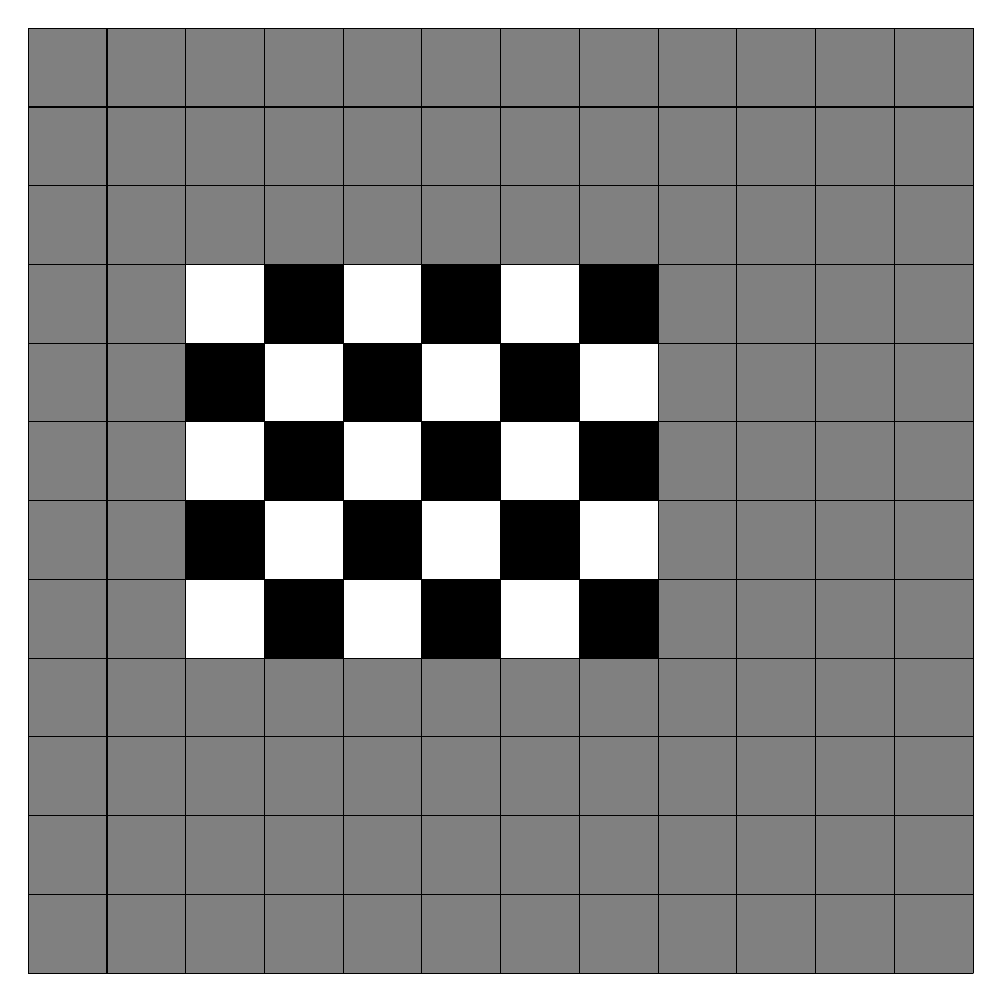
\begin{tikzpicture}
		\foreach \i in {-6, ..., 5}
			\foreach \j in {-6, ..., 5}
				\filldraw[gray] (\i, \j) rectangle + (1, 1);
		\foreach \i in {-4, ..., 1}
			\foreach \j in {-2, ..., 2}
			{
				\pgfmathparse{mod(\i+\j, 2) ? "black" : "white"}
				\edef\colour{\pgfmathresult}
				\filldraw[fill=\colour] (\i, \j) rectangle + (1, 1);
			}
		\draw[step=1] (-6, -6) grid (6, 6);
	\end{tikzpicture}
	\caption{Example of an image, that contains a rectangular region of interest with a checkerboard pattern.}
	\label{examplerROI}
\end{figure}

\paragraph{The statistical model}

Let $m, n \in \mathbb{N}$ and $c \in \mathbb{R} \setminus \{ 0 \}$. We assume we are given a noisy image following the statistical model
\begin{equation}\label{introductionstatmodel}
	F(i, j) = c + V(i, j) + \varepsilon_{i, j}
\end{equation}
for all $(i, j) \in \Omega \coloneqq \left\{ 1, \dots, m \right\} \times \left\{ 1, \dots, n \right\}$. For a grayscale image we take $c = 127.5$. We assume, that $V$ contains a rectangular region of interest with a checkerboard pattern, see figure \ref{examplerROI} for an example. This means, that the values of $V$ alternate between $c$ and $-c$ along the rows and columns of the region of interest. We call the set of all such images $\mathcal{V}_c^{m, n}$. We assume the noise terms $\varepsilon_{i, j} \sim \mathcal{N}(0, \sigma^2)$ to be i.i.d. normal distributed random variables for some $\sigma > 0$.

Notably, we make two simplifications. First, we assume the variance $\sigma$ of the noise terms to be known beforehand. Second, we ignore the limitations of grayscale images and let the images in our model take all values in the real numbers.

The image $F$ is the observed data we are given. The goal is to develop a statistical test for every pixel to determine whether or not the pixel belongs to the region of interest of $V$ and as such reconstructing the unknown $V$ from the noisy data. The pixel $(i, j)$ belonging to the ROI is equivalent to $\min \{ \norm{\Delta^+ V(i, j)}, \norm{\Delta^- V(i, j)} \} \neq 0$, where $\Delta^+$ and $\Delta^-$ denote the forward and backward discrete derivative operator, respectively. Thus, we get the null and alternative hypotheses
\begin{align*}
	H_0(i, j)&: \min \{ \norm{\Delta^+ V(i, j)}, \norm{\Delta^- V(i, j)} \} = 0 \\
	H_1(i, j)&: \min \{ \norm{\Delta^+ V(i, j)}, \norm{\Delta^- V(i, j)} \} \neq 0
\end{align*}
and the test statistic
\begin{equation*}
	T(i, j) \coloneqq \min \{ \norm{\Delta^+ F(i, j)}, \norm{\Delta^- F(i, j)} \}
\end{equation*}
for each pixel $(i, j) \in \Omega$. Based on these null hypotheses, we define the sets
\begin{equation*}
	\mathcal{H}_0(i, j) \coloneqq \left\{ V \in \mathcal{V}_c^{m, n} \mid \min \{ \norm{\Delta^+ V(i, j)}, \norm{\Delta^- V(i, j)} \} = 0 \right\}
\end{equation*}

Then $H_0(i, j)$ is true, if and only if $V \in \mathcal{H}_0(i, j)$. We use the notation $\mathbb{P}_V( \ldots )$ for the probability of an event for some \emph{fixed} image $V$ to analyze the error probabilities of the statistical test.

Let $V \in \mathcal{H}_0(i, j)$. Then $\norm{\Delta^+ V(i, j)} = $ or $\norm{\Delta^- V(i, j)} = 0$ and we can bound the statistical significance in the first case by
\begin{equation*}
	\mathbb{P}_V( T(i, j) \geq t ) \leq \mathbb{P}_V( \norm{\Delta^+ F(i, j)} \geq t )
\end{equation*}
and in the second case by
\begin{equation*}
	\mathbb{P}_V( T(i, j) \geq t ) \leq \mathbb{P}_V( \norm{\Delta^- F(i, j)} \geq t )
\end{equation*}

The right hand side of both inequalities is the same function, which can be computed explicitly. Using a trial and error algorithm, we can find a threshold $t_\alpha$ for a given statistical significance $\alpha \in ( 0, 1 )$, such that
\begin{equation*}
	\mathbb{P}_V( T(i, j) \geq t_\alpha ) \leq \alpha
\end{equation*}
for every $(i, j) \in \Omega$ and $V \in \mathcal{H}_0(i, j)$.

Since this is independent of the specific $V$, it holds for all images $V$ under which the null hypothesis for the pixel $(i, j)$ is true and thus we can bound the probability of falsely categorizing a background pixel as a foreground pixel by a given statistical significance $\alpha \in ( 0, 1 )$.

\paragraph{Main results}

After having established that we can ensure a given statistical significance in the statistical test, we aim at researching the changes of the statistical significance under morphological opening and closing.

To this end, let $\mathfrak{I} \in \{ 0, 1 \}^{m \times n}$ be a binary matrix and $\Psi \subseteq \mathbb{Z}^2$ be a structuring element. We denote by $\mathfrak{I} \circ \Psi$ the opening of the binary matrix $\mathfrak{I}$ by $\Psi$ and by $\mathfrak{I} \bullet \Psi$ the closing of the binary matrix $\mathfrak{I}$ by $\Psi$.

This notation allows us to write the main results of this paper. As the region of interest in our case is rectangular, it is natural to use a square structuring element. Using such a square structuring element yields an exponential improvement of the statistical significance after morphological opening. Applying morphological closing after opening will worsen the statistical significance, but only by a multiple. This yields an overall improvement of the statistical significance, when applying morphological opening and closing. These results are given in the following theorem.
\begin{theorem}
	Let $m, n \in \mathbb{N}$, $c \in \mathbb{R} \setminus \{ 0 \}$ and $\Omega = \left\{ 1, \dots, m \right\} \times \left\{ 1, \dots, m \right\}$. Assume we are given data
	\begin{equation*}
		F(i, j) = c + V(i, j) + \varepsilon_{i, j}
	\end{equation*}
	for all $(i, j) \in \Omega$, where the unknown $V$ contains a rectangular region of interest with a checkerboard pattern and $\varepsilon_{i, j} \sim \mathcal{N}(0, \sigma^2)$ are i.i.d. normal distributed random variables for some $\sigma > 0$.
	
	Let $\alpha \in (0, 1)$ and $t_\alpha$ be the threshold to ensure a statistical significance of $\alpha$ in the single pixel statistical test. Let $\mathfrak{I}_\alpha$ be the binary image defined by
	\begin{equation*}
		\mathfrak{I}_\alpha(i, j) = \mathds{1}_{ \{ T(i, j) \geq t_\alpha \} }
	\end{equation*}
	for all $(i, j) \in \Omega$.
	
	Let $k \in \mathbb{N}$ be odd. Let $\Phi_k = \{ -\frac{k - 1}{2}, -\frac{k - 3}{2}, \dots, \frac{k - 3}{2}, \frac{k - 1}{2} \}$ and $\Psi_k = \Phi_k \times \Phi_k$ be a structuring element. Let $(i, j) \in \Omega$ and $V \in \mathcal{H}_0(i, j)$.
	Then the following inequalities hold:
	\begin{align}
		\mathbb{P}_V( (\mathfrak{I}_\alpha \circ \Psi_k)(i, j) = 1 ) &\leq k \alpha^{\frac{k+1}{2}} \\
		\mathbb{P}_V( ( (\mathfrak{I}_\alpha \circ \Psi_k) \bullet \Psi_k)(i, j) = 1 ) &\leq k^3 \alpha^{\frac{k+1}{2}}
	\end{align}
\end{theorem}

While these results hold only in our simplified model, it is worth noting, that our model and statistical test exhibit high similarities to widely used techniques in automated fingerprint recognition.

\paragraph{Outline of the paper}

In section \ref{sectiondefinitions} we will introduce mathematical definitions of the aforementioned images and properties. With the introduced terminology we develop a statistical test for every pixel to determine whether or not it is part of the region of interest in section \ref{sectionstatisticalmodel}. After having established the statistical test, we proof in section \ref{sectionstatisticalsignificance} that we can ensure a given statistical significance and analyze the power of the statistical test in section \ref{sectionpower}. Afterwards, in section \ref{sectionmorphologicaloperations} we introduce the two morphological operators, that we study in this paper, along with some examples of their application. From there, we proceed to proof the main theorems of this paper in section \ref{sectionmainresults}.

\newpage

\section{Testing for a rectangular region of interest}

\subsection{Definitions}\label{sectiondefinitions}

As discussed before, we limit our research to a simplified model. We assume that the noise-free image $V$ in our statistical model has a rectangular region of interest with a checkerboard pattern, cp. equation \eqref{introductionstatmodel} and figure \ref{examplerROI}. In the following we give mathematical definitions of these properties.

\begin{definition}
	Let $m, n \in \mathbb{N}$ and $V \in \mathbb{R}^{m \times n}$. Let $(\kappa_1, \lambda_1), (\kappa_2, \lambda_2)$ be two pairs of indices with $1 \leq \kappa_1 \leq \kappa_2 \leq m$ and $1 \leq \lambda_1 \leq \lambda_2 \leq m$, such that
	\begin{equation}\label{eqrROI}
		V(i, j) \neq 0 \textrm{ if and only if } (i, j) \in \{ \kappa_1, \dots, \kappa_2 \} \times \{ \lambda_1, \dots, \lambda_2 \}
	\end{equation}
	We call $\varLambda = \{ \kappa_1, \dots, \kappa_2 \} \times \{ \lambda_1, \dots, \lambda_2 \}$ a \emph{rectangular region of interest (rROI)} and say that $V$ contains the rROI $\varLambda$.
	
	Furthermore, we call $(\kappa_1, \lambda_1)$ the \emph{top left corner} and $(\kappa_2, \lambda_2)$ the \emph{bottom right corner} of $\varLambda$.
\end{definition}

\begin{definition}
	Let $m, n \in \mathbb{N}$ and $c \in \mathbb{R} \setminus \{ 0 \}$. Let $V \in \mathbb{R}^{m \times n}$ be a matrix, that only takes values in the set $\{ 0, \pm c \}$, i.e. $V \in \{ 0, \pm c \}^{m \times n}$. Let $V$ contain a rectangular region of interest $\varLambda$ and let $(\kappa_1, \lambda_1)$ be the top left corner of $\varLambda$. We say that $\varLambda$ has a \emph{checkerboard pattern}, if the equivalence
	\begin{equation}\label{eqcheckerboard}
		V(i, j) = c \Leftrightarrow i + j \equiv \kappa_1 + \lambda_1 \mod 2
	\end{equation}
	holds for all $(i, j) \in \varLambda$.
\end{definition}

\begin{remark}
	Relation \eqref{eqcheckerboard} implies $V(\kappa_1, \lambda_1) = c$. Furthermore, we have assumed that $V$ only takes values in $\{ 0, \pm c \}$. Also, by assumption $V$ contains a rROI, which implies $V(i,j) \neq 0$, if and only if $(i, j) \in \varLambda$. This yields
	\begin{equation*}
		V(i, j) = - c \Leftrightarrow i + j \not\equiv \kappa_1 + \lambda_1 \mod 2
	\end{equation*}
	for all $(i, j) \in \varLambda$.
\end{remark}

Hence, the top left corner of $V$ takes the value $c$ and then the values of $V$ alternate between $+c$ and $-c$ along the rows and columns of $\varLambda$. This is similar to the classical checkerboard pattern.

\begin{definition}
	Let $m, n \in \mathbb{N}$ and $c \in \mathbb{R} \setminus \{ 0 \}$. We define $\mathcal{V}_c^{m, n}$ to be the set of all matrices, that only take values in $\{ 0, \pm c \}$ and that contain a rROI with a checkerboard pattern, i.e. all matrices  $V \in \{ 0, \pm c \}^{m \times n}$, that fulfill equivalences \eqref{eqrROI} and \eqref{eqcheckerboard} for some $1 \leq \kappa_1 \leq \kappa_2 \leq m$ and $1 \leq \lambda_1 \leq \lambda_2 \leq n$.
\end{definition}

\begin{remark}
	Any matrix $V \in \mathcal{V}_c^{m, n}$ is uniquely defined by the top left and bottom right corner of $\varLambda$. Hence, a rROI $\varLambda = \{ \kappa_1, \dots, \kappa_2 \} \times \{ \lambda_1, \dots, \lambda_2 \}$ corresponds to a unique element $V \in \mathcal{V}_c^{m, n}$, that contains the rROI $\varLambda$.
\end{remark}

In figure \ref{examplerROItlcbrc} we see an example of such a matrix. To visualize these types of matrices, we take $c = 127.5$ and plot the grayscale image $V + c$. Thus, gray pixels represent $V = 0$, white pixels represent $V = c$ and black pixels represent $V = - c$.

% Draw example of a matrix with a rROI with a checkerboard pattern:
\begin{figure}[h]
	\centering
	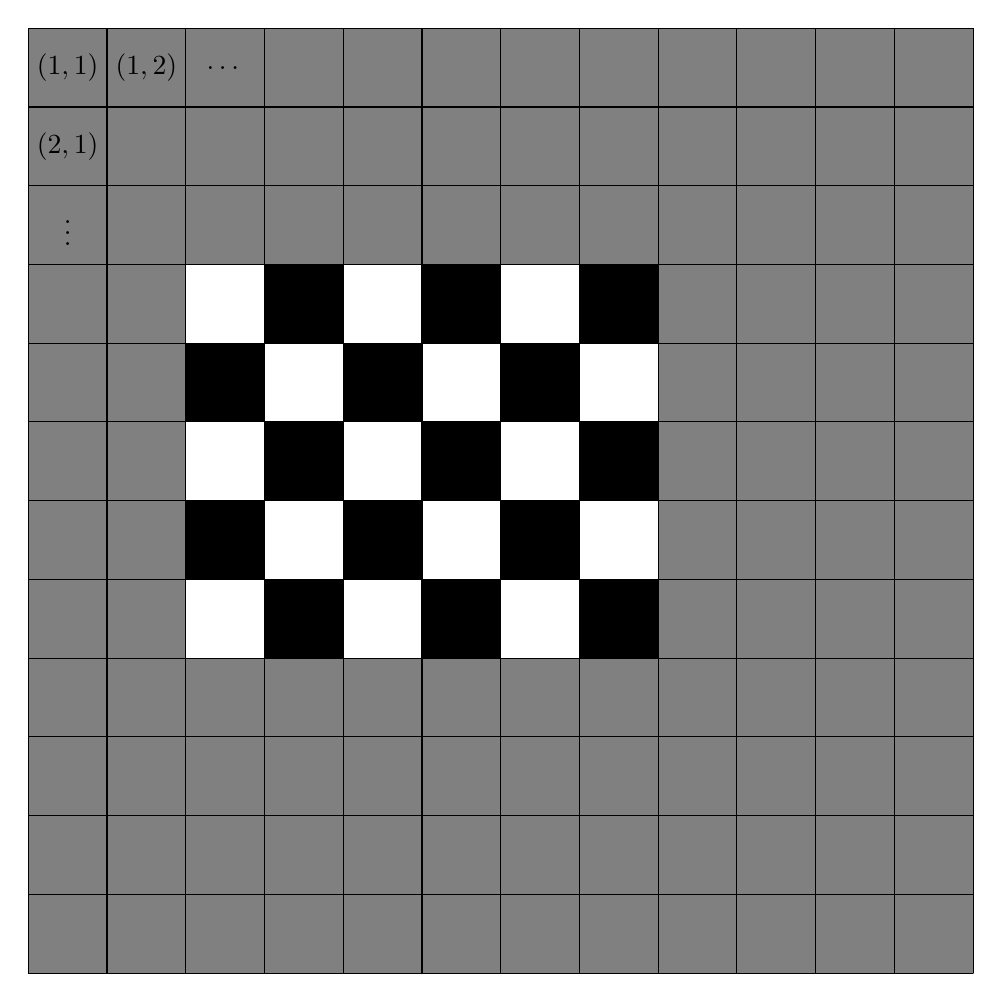
\begin{tikzpicture}
		\foreach \i in {-6, ..., 5}
			\foreach \j in {-6, ..., 5}
				\filldraw[gray] (\i, \j) rectangle + (1, 1);
		\foreach \i in {-4, ..., 1}
			\foreach \j in {-2, ..., 2}
			{
				\pgfmathparse{mod(\i+\j, 2) ? "black" : "white"}
				\edef\colour{\pgfmathresult}
				\filldraw[fill=\colour] (\i, \j) rectangle + (1, 1);
			}
		\draw[step=1] (-6, -6) grid (6, 6);
		\node at (-5.5, 5.5) {$(1, 1)$};
		\node at (-4.5, 5.5) {$(1, 2)$};
		\node at (-3.5, 5.5) {$\dots$};
		\node at (-5.5, 4.5) {$(2, 1)$};
		\node at (-5.5, 3.5) {$\vdots$};
	\end{tikzpicture}
	\caption{Example of a matrix, that contains a rROI with a checkerboard pattern. The top left corner of the rROI is $(4, 3)$ and the bottom right corner is $(8, 8)$. Here we have $m = n = 12$.}
	\label{examplerROItlcbrc}
\end{figure}

The goal of the previous definitions was to formalize the objects of study of this paper: Images, that have a rectangular region of interest with a black \& white checkerboard pattern surrounded by a constant gray background. We also need the forward and backward discrete derivative operator to establish our statistical test. As a reminder, we give the definition of these operators.

\begin{definition}
	Let $m, n \in \mathbb{N}$ and let $V \in \mathbb{R}^{m \times n}$. Define the set of possible indices $\Omega \coloneqq \{ 1, \dots, m \} \times \{ 1, \dots, m \}$. Let $(i, j) \in \Omega$. The \textit{forward and backward discrete derivative of $V$ evaluated at $(i, j)$} are defined as
	\begin{equation}
		\Delta^+ V(i, j) =
		\begin{pmatrix}
			V(i + 1, j) - V(i, j) \\
			V(i, j + 1) - V(i, j)
		\end{pmatrix}
	\end{equation}
	and
	\begin{equation}
		\Delta^- V(i, j) =
		\begin{pmatrix}
			V(i - 1, j) - V(i, j) \\
			V(i, j - 1) - V(i, j)
		\end{pmatrix}
	\end{equation}
	respectively. To adjust to boundary issues, we use a periodic boundary condition, i.e. $V(i, j) = V(i \mod m, j \mod n)$ for all $(i, j) \in \mathbb{Z}^2$.
\end{definition}

The following lemma shows, that the euclidean norm of these operators for matrices $V \in \mathcal{V}_c^{m, n}$ can only take specific values.

\begin{lemma}\label{lemsetD}
	Let $m, n \in \mathbb{N}$ and $c \in \mathbb{R} \setminus \{ 0 \}$. Let $V \in \mathcal{V}_c^{m, n}$. For any $(i, j) \in \Omega$ we have
	\begin{equation}
		\norm{\Delta^+ V(i, j)}, \norm{\Delta^- V(i, j)} \in \{ 0, c, \sqrt{2} c, \sqrt{5} c, \sqrt{8} c \}
	\end{equation}
\end{lemma}
\begin{proof}
	Let $(i, j) \in \Omega$. We have assumed, that $V \in \mathcal{V}_c^{m, n}$. Thus, $V$ only takes values in $\{ 0, \pm c \}$ and we obtain $\Delta^+ V(i, j), \Delta^- V(i, j) \in \{ 0, \pm c, \pm 2 c \}^2$. Taking the euclidean norm of all possible combinations yields
	\begin{equation*}
		\norm{\Delta^+ V(i, j)}, \norm{\Delta^- V(i, j)} \in \{ 0, c, 2 c, \sqrt{2} c, \sqrt{5} c, \sqrt{8} c \}
	\end{equation*}
	
	We can narrow this list down even more. By assumption, $V$ contains a rectangular region of interest $\varLambda$ with a checkerboard pattern. This only allows the following combinations of $\abs{V(i + 1, j) - V(i, j)}$ and $\abs{V(i, j + 1) - V(i, j)}$:
	\begin{table}[h]
		\centering
		\resizebox{\textwidth}{!}{
			\begin{tabular}{c|c|c|c}
				\textbf{Position of pixels} $\mathbf{(i, j)}$, $\mathbf{(i + 1, j)}$, $\mathbf{(i, j + 1)}$ & $\mathbf{\abs{V(i + 1, j) - V(i, j)}}$ & $\mathbf{\abs{V(i, j + 1) - V(i, j)}}$ & $\mathbf{\norm{\Delta^+ V(i, j)}}$ \\
				\hline
				$(i, j), (i + 1, j), (i, j + 1) \notin \varLambda$ & $0$ & $0$ & $0$ \\
				\hline
				$(i, j), (i + 1, j) \notin \varLambda$ and $(i, j + 1) \in \varLambda$ & $0$ & $c$ & $c$ \\
				\hline
				$(i, j), (i, j + 1) \notin \varLambda$ and $(i + 1, j) \in \varLambda$ & $c$ & $0$ & $c$ \\
				\hline
				$(i, j) \in \varLambda$ and $(i + 1, j), (i, j + 1) \notin \varLambda$ & $c$ & $c$ & $\sqrt{2} c$ \\
				\hline
				$(i, j), (i + 1, j) \in \varLambda$ and $(i, j + 1) \notin \varLambda$ & $2 c$ & $c$ & $\sqrt{5} c$ \\
				\hline
				$(i, j), (i, j + 1) \in \varLambda$ and $(i + 1, j) \notin \varLambda$ & $c$ & $2 c$ & $\sqrt{5} c$ \\
				\hline
				$(i, j), (i + 1, j), (i, j + 1) \in \varLambda$ & $2 c$ & $2 c$ & $\sqrt{8} c$ \\
			\end{tabular}
		}
	\caption{Possible locations of the pixels $(i, j)$, $(i + 1, j)$, $(i, j + 1)$ and the corresponding values of $\abs{V(i + 1, j) - V(i, j)}$ and $\abs{V(i, j + 1) - V(i, j)}$.}
	\label{tablediscretederivativevalues}
	\end{table}
	
	Other cases are not possible and thus $\norm{\Delta^+ V(i, j)} \in \{ 0, c, \sqrt{2} c, \sqrt{5} c, \sqrt{8} c \}$. By a similar deduction, we also obtain $\norm{\Delta^- V(i, j)} \in \{ 0, c, \sqrt{2} c, \sqrt{5} c, \sqrt{8} c \}$.
	
	This finishes the proof.
\end{proof}

\newpage

\subsection{Statistical model}\label{sectionstatisticalmodel}

After having established the definitions needed for our statistical model, we can proceed to develop a statistical test, that categorizes pixels as fore- or background.

Let $m, n \in \mathbb{N}$, $c \in \mathbb{R} \setminus \{ 0 \}$ and $\Omega = \left\{ 1, \dots, m \right\} \times \left\{ 1, \dots, n \right\}$. Assume we are given noisy data
\begin{equation}\label{image}
	F(i, j) = c + V(i, j) + \varepsilon_{i, j}
\end{equation}
for all $(i, j) \in \Omega$, where $V \in \mathcal{V}_c^{m, n}$ is unknown and $\varepsilon_{i, j} \sim \mathcal{N}(0, \sigma^2)$ are i.i.d. normal distributed random variables for some $\sigma > 0$.

Let $\varLambda$ be the rectangular region of interest contained in $V$. We aim to find a statistical test to determine for each individual pixel whether $(i, j) \in \varLambda$ or $(i, j) \notin \varLambda$.

From the assumption, that $V$ contains a rROI, it follows, that $V(i, j) = 0$ if and only if $(i, j) \notin \varLambda$. Let $(\kappa_1, \lambda_1)$ and $(\kappa_2, \lambda_2)$ be the top left and bottom right corner of $\varLambda$, respectively. Now, if $(i, j) \notin \varLambda$, it follows that $i \notin \{ \kappa_1, \dots, \kappa_2 \}$ or $j \notin \{ \lambda_1, \dots, \lambda_2 \}$. We have to distinguish four cases here:
\begin{align*}
	i < \kappa_1 &\Rightarrow (i, j - 1) \notin \varLambda \textrm{ and } (i - 1, j) \notin \varLambda \\
	&\Rightarrow V(i, j - 1) = V(i - 1, j) = 0 \\
	j < \lambda_1 &\Rightarrow (i - 1, j) \notin \varLambda \textrm{ and } (i, j - 1) \notin \varLambda \\
	&\Rightarrow V(i - 1, j) = V(i, j - 1) = 0 \\
	i > \kappa_2 &\Rightarrow (i, j + 1) \notin \varLambda \textrm{ and } (i + 1, j) \notin \varLambda \\
	&\Rightarrow V(i, j + 1) = V(i + 1, j) = 0 \\
	j > \lambda_2 &\Rightarrow (i + 1, j) \notin \varLambda \textrm{ and } (i, j + 1) \notin \varLambda \\
	&\Rightarrow V(i + 1, j) = V(i, j + 1) = 0
\end{align*}

We see, that in the first two cases, we have $\norm{\Delta^- V(i, j)} = 0$. In the latter two cases, we get $\norm{\Delta^+ V(i, j)} = 0$. Thus, if $(i, j) \notin \varLambda$, it follows that $\min \{ \norm{\Delta^+ V(i, j)}, \norm{\Delta^- V(i, j)} \} = 0$.

On the other hand, we have assumed, that $\varLambda$ has a checkerboard pattern. Thus $\norm{\Delta^- V(i, j)}, \norm{\Delta^+ V(i, j)} \neq 0$ for $(i, j) \in \varLambda$. This yields the equivalence
\begin{equation*}
	(i, j) \notin \varLambda \Leftrightarrow \min \{ \norm{\Delta^+ V(i, j)}, \norm{\Delta^- V(i, j)} \} = 0
\end{equation*}

Since our goal is to test for $(i, j) \in \varLambda$, we define a null hypothesis for each individual pixel:
\begin{equation*}
	H_0(i, j): \min \{ \norm{\Delta^+ V(i, j)}, \norm{\Delta^- V(i, j)} \} = 0
\end{equation*}

We do not know the actual values of $V$, which makes $\Delta^+ V$ and $\Delta^- V$ non-observable. Since we are given noisy data, we use this noisy data for our test statistic and test for each individual pixel $(i, j)$ the null hypothesis
\begin{equation}\label{nullhypothesis}
	H_0(i, j): \min \{ \norm{\Delta^+ V(i, j)}, \norm{\Delta^- V(i, j)} \} = 0
\end{equation}
against the alternative hypothesis
\begin{equation}\label{alternativehypothesis}
	H_1(i, j): \min \{ \norm{\Delta^+ V(i, j)}, \norm{\Delta^- V(i, j)} \} \neq 0
\end{equation}
using the test statistic
\begin{equation}\label{teststatistic}
	T(i, j) \coloneqq \min \{ \norm{\Delta^+ F(i, j)}, \norm{\Delta^- F(i, j)} \}
\end{equation}

The pixels the can be categorized by rejecting the null hypothesis, i.e. classifying the pixel $(i, j)$ as foreground, if $T(i, j) \geq t$ for some threshold $t \in \mathbb{R}^+$. How the threshold should be chosen will be examined in section \ref{sectionstatisticalsignificance}.

For convenience, we want to define some subsets of $\mathcal{V}_c^{m, n}$. For every $(i, j) \in \Omega$ we define the set of images, for which the null hypothesis $H_0(i, j)$ is true as
\begin{equation}
	\mathcal{H}_0(i, j) \coloneqq \left\{ V \in \mathcal{V}_c^{m, n} \mid \min \{ \norm{\Delta^+ V(i, j)}, \norm{\Delta^- V(i, j)} \} = 0 \right\}
\end{equation}

Then $H_0(i, j)$ is true, if and only if $V \in \mathcal{H}_0(i, j)$. Furthermore, we define two subsets of this set as
\begin{align}
	\mathcal{H}_0^+(i, j) &\coloneqq \left\{ V \in \mathcal{V}_c^{m, n} \mid \norm{\Delta^+ V(i, j)} = 0 \right\} \label{setH0+} \\
	\mathcal{H}_0^-(i, j) &\coloneqq \left\{ V \in \mathcal{V}_c^{m, n} \mid \norm{\Delta^- V(i, j)} = 0 \right\} \label{setH0-}
\end{align}

Then $\mathcal{H}_0(i, j) = \mathcal{H}_0^+(i, j) \cup \mathcal{H}_0^-(i, j)$, where the union is not necessarily disjoint.

\newpage

\subsection{Analysis of the statistical significance}\label{sectionstatisticalsignificance}

After having established our hypotheses and test statistic, we want to examine the choice of the threshold $t \in \mathbb{R}^+$ in the testing procedure. We reject the null hypothesis, if $T(i, j) \geq t$ for some threshold $t \in \mathbb{R}^+$. We want to choose $t$ such, that the probability of falsely classifying a background pixel as foreground is bound to a given statistical significance $\alpha \in (0, 1)$. Such a threshold will be denoted as $t_\alpha$.

As a reminder, we use the notation $\mathbb{P}_V( \ldots )$ for the probability of an event for some \emph{fixed} image $V$. This will allow us to analyze the probabilites of falsely categorizing a pixel. Using this notation, we want to find a threshold $t_\alpha$, such that $\mathbb{P}_V( T(i, j) \geq t_\alpha ) \leq \alpha$ for every $V \in \mathcal{H}_0(i, j)$. A first step towards finding such a threshold is the following lemma.

\begin{lemma}\label{lemtypeIbound}
	Let $(i, j) \in \Omega$ and $t \in \mathbb{R}^+$. Assume that $F$ follows the statistical model given in \eqref{image} and let $T(i, j)$ be defined as in \eqref{teststatistic}. Let $V \in \mathcal{V}_c^{m, n}$. Then
	\begin{equation}\label{eqtypeIbound}
		\mathbb{P}_V( T(i, j) \geq t ) \leq \min \left\{ \mathbb{P}_V( \norm{\Delta^+ F(i, j)} \geq t ), \mathbb{P}_V( \norm{\Delta^- F(i, j)} \geq t ) \right\}
	\end{equation}
\end{lemma}
\begin{proof}
	Let $t \in \mathbb{R}^+$. On the one hand, we have
	\begin{align*}
		\mathbb{P}_V( T(i, j) \geq t ) &= \mathbb{P}_V( \min \{ \norm{\Delta^+ F(i, j)}, \norm{\Delta^- F(i, j)} \} \geq t ) \\
		&= \mathbb{P}_V( \{ \norm{\Delta^+ F(i, j)} \geq t \} \cap \{ \norm{\Delta^- F(i, j)} \geq t \} ) \\
		&\leq \mathbb{P}_V( \norm{\Delta^+ F(i, j)} \geq t )
	\end{align*}
	
	On the other hand, we obtain analogously
	\begin{equation*}
		\mathbb{P}_V( T(i, j) \geq t ) \leq \mathbb{P}_V( \norm{\Delta^- F(i, j)} \geq t )
	\end{equation*}
	
	Combining these two inequalities yields the result and thus finishes the proof of the lemma.
\end{proof}

The second step is given in the following theorem, where we calculate the cumulative distribution functions of $\mathbb{P}_V( \norm{\Delta^+ F(i, j)} \leq t )$ for $V \in \mathcal{H}_0^+(i, j)$ and $\mathbb{P}_V( \norm{\Delta^- F(i, j)} \leq t )$ for $V \in \mathcal{H}_0^-(i, j)$, which turn out to be the same.

\begin{theorem}\label{thmeqcdf}
	Let $(i, j) \in \Omega$ and $t \in \mathbb{R}^+$. Assume that $F$ follows the statistical model given in \eqref{image}. Let $V_1 \in \mathcal{H}_0^+(i, j)$ and $V_2 \in \mathcal{H}_0^-(i, j)$. Then
	\begin{equation}\label{eqprobequality}
		\mathbb{P}_{V_1}( \norm{\Delta^+ F(i, j)} \leq t ) = p(t) = \mathbb{P}_{V_2}( \norm{\Delta^- F(i, j)} \leq t )
	\end{equation}
	where
	\begin{equation}\label{eqcdf}
		\begin{aligned}
			p(t) &\coloneqq \frac{1}{\sqrt{3}} \left( \frac{3}{2} - \frac{3}{2} \exp \left( - \frac{t^2}{3 \sigma^2} \right) I_0 \left( \frac{t^2}{6 \sigma^2} \right) \right) - \sqrt{3} \\
			&\quad - \frac{2 - \sqrt{3}}{2} Q_1 \left( \frac{2 - \sqrt{3}}{6} \sqrt{\frac{t}{\sigma}}, \frac{2 + \sqrt{3}}{6} \sqrt{\frac{t}{\sigma}} \right) \\
			&\quad + \frac{2 + \sqrt{3}}{2} Q_1 \left( \frac{2 + \sqrt{3}}{6} \sqrt{\frac{t}{\sigma}}, \frac{2 - \sqrt{3}}{6} \sqrt{\frac{t}{\sigma}} \right)
		\end{aligned}
	\end{equation}
	with $I_0$ being the modified Bessel function of the first kind and $Q_M$ denoting the Marcum $Q$-function.
\end{theorem}
\begin{proof}
	We start by proving the first equality of equation \eqref{eqprobequality}. By assumption, $V_1 \in \mathcal{H}_0^+(i, j)$ and thus $\norm{\Delta^+ V_1(i, j)} = 0$. By definition of $\Delta^+$ we get the equivalence
	\begin{equation*}
		\norm{\Delta^+ V_1(i, j)} = 0 \Leftrightarrow V_1(i + 1, j) - V_1(i, j) = V_1(i, j + 1) - V_1(i, j) = 0
	\end{equation*}
	
	We write out the term $\mathbb{P}_{V_1}( \norm{\Delta^+ F(i, j)} \leq t )$, which we call $q(t)$, and use the equivalence above to get
	\begin{align*}
		q(t) &\coloneqq \mathbb{P}_{V_1}( \norm{\Delta^+ F(i, j)} \leq t ) \\
		&= \mathbb{P}_{V_1}\big( (c + V_1(i + 1, j) + \varepsilon_{i + 1, j} - c - V_1(i, j) - \varepsilon_{i, j})^2 \\
		&\quad + (c + V_1(i, j + 1) + \varepsilon_{i, j + 1} - c - V_1(i, j) - \varepsilon_{i, j})^2 \leq t^2 \big) \\
		&= \mathbb{P}_{V_1}\left( (\varepsilon_{i + 1, j} - \varepsilon_{i, j})^2 + (\varepsilon_{i, j + 1} - \varepsilon_{i, j})^2 \leq t^2 \right) \\
		&= \mathbb{P}\left( (\varepsilon_{i + 1, j} - \varepsilon_{i, j})^2 + (\varepsilon_{i, j + 1} - \varepsilon_{i, j})^2 \leq t^2 \right)
	\end{align*}
	where we dropped the index $V_1$, since the probability does no longer depend on $V_1$.
	
	Assuming the common term $\varepsilon_{i, j}$ to be constant and by defining
	\begin{align*}
		X_1 &= \varepsilon_{i + 1, j} - \varepsilon_{i, j} \sim \mathcal{N}(- \varepsilon_{i, j}, \sigma^2) \\
		X_2 &= \varepsilon_{i, j + 1} - \varepsilon_{i, j} \sim \mathcal{N}(- \varepsilon_{i, j}, \sigma^2)
	\end{align*}
	we obtain
	\begin{equation*}
		q(t) = \mathbb{P}\left( \sqrt{\left( \frac{X_1}{\sigma} \right)^2 + \left( \frac{X_2}{\sigma} \right)^2} \leq \frac{t}{\sigma} \right)
	\end{equation*}
	
	This shows, that the square root inside has a non-central Chi distribution with two degrees of freedom and non-centrality parameter
	\begin{equation*}
		\lambda = \sqrt{\left( \frac{- \varepsilon_{i, j}}{\sigma} \right)^2 + \left( \frac{- \varepsilon_{i, j}}{\sigma} \right)^2} = \frac{\sqrt{2} \abs{\varepsilon_{i, j}}}{\sigma}
	\end{equation*}
	and hence
	\begin{equation*}
		\sqrt{\left( \frac{X_1}{\sigma} \right)^2 + \left( \frac{X_2}{\sigma} \right)^2} \sim \chi_2 \left( \frac{\sqrt{2} \abs{\varepsilon_{i, j}}}{\sigma} \right)
	\end{equation*}
	
	Up until this point we assumed $\varepsilon_{i, j}$ to be constant, but it is a normal distributed random variable with zero mean and standard deviation $\sigma$. Thus, we have a compound probability distribution:
	\begin{align*}
		q(t) &= \mathbb{P}\left( \sqrt{\left( \frac{X_1}{\sigma} \right)^2 + \left( \frac{X_2}{\sigma} \right)^2} \leq \frac{t}{\sigma} \right) \\
		&= \int_0^\frac{t}{\sigma} \int_0^\infty \underbrace{x \exp \left( - \frac{x^2}{2} - \frac{\eta^2}{\sigma^2} \right) I_0 \left( \frac{\sqrt{2} \eta}{\sigma} x \right)}_{\textrm{pdf of} \ \chi_2 \left( \frac{\sqrt{2} \eta}{\sigma} \right) \ \textrm{for fixed} \ \eta} \underbrace{\frac{2}{\sqrt{2 \pi \sigma^2}} \exp \left( - \frac{\eta^2}{2 \sigma^2} \right)}_{\textrm{pdf of absolute value of} \ \mathcal{N}(0, \sigma^2)} \mathrm{d}\eta \mathrm{d}x \\
		&= \frac{2}{\sqrt{2 \pi \sigma^2}} \int_0^\frac{t}{\sigma} x \exp \left( - \frac{x^2}{2} \right) \int_0^\infty \exp \left( - \frac{3}{2 \sigma^2} \eta^2 \right) I_0 \left( \frac{\sqrt{2} x}{\sigma} \eta \right) \mathrm{d}\eta \mathrm{d}x
	\end{align*}
	
	where $I_0$ is the modified Bessel function of the first kind. We can solve the inner integral first. For $\mathrm{Re} \ \nu > -1$, $\mathrm{Re} \ \alpha > 0$ the following equality holds\cite{TISP}.
	\begin{equation}\label{eqintbessel}
		\int_0^\infty \exp \left( - \alpha x^2 \right) I_\nu ( \beta x ) \mathrm{d}x = \frac{\sqrt{\pi}}{2 \sqrt{\alpha}} \exp \left( \frac{\beta^2}{8 \alpha} \right) I_{\frac{1}{2} \nu} \left( \frac{\beta^2}{8 \alpha} \right)
	\end{equation}
	
	In our case, we have $\nu = 0$, $\alpha = \frac{3}{2 \sigma^2}$ and $\beta = \frac{\sqrt{2} x}{\sigma}$, which yields
	\begin{align*}
		\int_0^\infty \exp \left( - \frac{3}{2 \sigma^2} \eta^2 \right) I_0 \left( \frac{\sqrt{2} x}{\sigma} \eta \right) \mathrm{d}\eta &= \frac{\sqrt{\pi}}{2 \sqrt{\frac{3}{2 \sigma^2}}} \exp \left( \frac{\frac{2 x^2}{\sigma^2}}{8 \frac{3}{2 \sigma^2}} \right) I_0 \left( \frac{\frac{2 x^2}{\sigma^2}}{8 \frac{3}{2 \sigma^2}} \right) \\
		&= \frac{\sqrt{\pi} \sigma}{\sqrt{6}} \exp \left( \frac{x^2}{6} \right) I_0 \left( \frac{x^2}{6} \right)
	\end{align*}
	
	Plugging this in, we obtain
	\begin{align*}
		q(t) &= \frac{2}{\sqrt{2 \pi \sigma^2}} \int_0^\frac{t}{\sigma} x \exp \left( - \frac{x^2}{2} \right) \frac{\sqrt{\pi} \sigma}{\sqrt{6}} \exp \left( \frac{x^2}{6} \right) I_0 \left( \frac{x^2}{6} \right) \mathrm{d}x \\
		&= \frac{1}{\sqrt{3}} \int_0^\frac{t}{\sigma} x \exp \left( - \frac{x^2}{2} \right) \exp \left( \frac{x^2}{6} \right) I_0 \left( \frac{x^2}{6} \right) \mathrm{d}x \\
		&= \frac{1}{\sqrt{3}} \int_0^\frac{t}{\sigma} x \exp \left( - \frac{x^2}{3} \right) I_0 \left( \frac{x^2}{6} \right) \mathrm{d}x
	\end{align*}
	
	To proceed, we need to integrate by parts to replace the modified Bessel function $I_0$ with order zero by a modified Bessel function $I_1$ with order one.
	\begin{align*}
		q(t) &= \frac{1}{\sqrt{3}} \left[ - \frac{3}{2} \exp \left( - \frac{x^2}{3} \right) I_0 \left( \frac{x^2}{6} \right) \right]_0^\frac{t}{\sigma} + \frac{1}{2 \sqrt{3}} \int_0^\frac{t}{\sigma} \exp \left( - \frac{x^2}{3} \right) x I_1 \left( \frac{x^2}{6} \right) \mathrm{d}x \\
		&= \frac{1}{\sqrt{3}} \left( \frac{3}{2} - \frac{3}{2} \exp \left( - \frac{t^2}{3 \sigma^2} \right) I_0 \left( \frac{t^2}{6 \sigma^2} \right) \right) + \frac{1}{2 \sqrt{3}} \int_0^\frac{t}{\sigma} \exp \left( - \frac{x^2}{3} \right) x I_1 \left( \frac{x^2}{6} \right) \mathrm{d}x
	\end{align*}
	
	In the next step we substitute $y = x^2$ in the remaining integral, which leaves us with
	\begin{equation*}
		q(t) = \frac{1}{\sqrt{3}} \left( \frac{3}{2} - \frac{3}{2} \exp \left( - \frac{t^2}{3 \sigma^2} \right) I_0 \left( \frac{t^2}{6 \sigma^2} \right) \right) + \frac{1}{4 \sqrt{3}} \int_0^\frac{t}{\sigma} \exp \left( - \frac{y}{3} \right) I_1 \left( \frac{y}{6} \right) \mathrm{d}y
	\end{equation*}
	
	We want to solve the remaining integral. Let $p \neq b$ and $s = \sqrt{p^2 - b^2}$, $u = \sqrt{a (p - s)}$ and $v = \sqrt{a (p + s)}$. Then\cite{IntQFunction}
	\begin{equation}\label{eqintmarcum}
		\int_0^a \exp(-p x) I_M ( b x ) \mathrm{d}x = \frac{1}{s b^M} \left( (p - s)^M ( 1 - Q_M(u, v) ) - (p + s)^M ( 1 - Q_M(v, u) ) \right)
	\end{equation}
	where $Q_M$ denotes the Marcum $Q$-function. The Marcum $Q$-function is only defined for $M \geq 1$, which made the integration by parts necessary. Applying this equation with $M = 1$ to the integral yields
	\begin{align*}
		\int_0^\frac{t}{\sigma} \exp \left( - \frac{y}{3} \right) I_1 \left( \frac{y}{6} \right) \mathrm{d}y &= \frac{1}{\frac{1}{2 \sqrt{3}} \frac{1}{6}} \frac{2 - \sqrt{3}}{6} \left( 1 - Q_1 \left( \frac{2 - \sqrt{3}}{6} \sqrt{\frac{t}{\sigma}}, \frac{2 + \sqrt{3}}{6} \sqrt{\frac{t}{\sigma}} \right) \right) \\
		&\quad - \frac{1}{\frac{1}{2 \sqrt{3}} \frac{1}{6}} \frac{2 + \sqrt{3}}{6} \left( 1 - Q_1 \left( \frac{2 + \sqrt{3}}{6} \sqrt{\frac{t}{\sigma}}, \frac{2 - \sqrt{3}}{6} \sqrt{\frac{t}{\sigma}} \right) \right) \\
		&= 2 \sqrt{3} (2 - \sqrt{3}) \left( 1 - Q_1 \left( \frac{2 - \sqrt{3}}{6} \sqrt{\frac{t}{\sigma}}, \frac{2 + \sqrt{3}}{6} \sqrt{\frac{t}{\sigma}} \right) \right) \\
		&\quad - 2 \sqrt{3} (2 + \sqrt{3}) \left( 1 - Q_1 \left( \frac{2 + \sqrt{3}}{6} \sqrt{\frac{t}{\sigma}}, \frac{2 - \sqrt{3}}{6} \sqrt{\frac{t}{\sigma}} \right) \right)
	\end{align*}
	
	Plugging this in, we obtain the final result
	\begin{align*}
		q(t) &= \frac{1}{\sqrt{3}} \left( \frac{3}{2} - \frac{3}{2} \exp \left( - \frac{t^2}{3 \sigma^2} \right) I_0 \left( \frac{t^2}{6 \sigma^2} \right) \right) + \frac{1}{4 \sqrt{3}} \int_0^\frac{t}{\sigma} \exp \left( - \frac{y}{3} \right) I_1 \left( \frac{y}{6} \right) \mathrm{d}y \\
		&= \frac{1}{\sqrt{3}} \left( \frac{3}{2} - \frac{3}{2} \exp \left( - \frac{t^2}{3 \sigma^2} \right) I_0 \left( \frac{t^2}{6 \sigma^2} \right) \right) \\
		&\quad + \frac{2 \sqrt{3}}{4 \sqrt{3}} (2 - \sqrt{3}) \left( 1 - Q_1 \left( \frac{2 - \sqrt{3}}{6} \sqrt{\frac{t}{\sigma}}, \frac{2 + \sqrt{3}}{6} \sqrt{\frac{t}{\sigma}} \right) \right) \\
		&\quad - \frac{2 \sqrt{3}}{4 \sqrt{3}} (2 + \sqrt{3}) \left( 1 - Q_1 \left( \frac{2 + \sqrt{3}}{6} \sqrt{\frac{t}{\sigma}}, \frac{2 - \sqrt{3}}{6} \sqrt{\frac{t}{\sigma}} \right) \right) \\
		&= \frac{1}{\sqrt{3}} \left( \frac{3}{2} - \frac{3}{2} \exp \left( - \frac{t^2}{3 \sigma^2} \right) I_0 \left( \frac{t^2}{6 \sigma^2} \right) \right) - \sqrt{3} \\
		&\quad - \frac{2 - \sqrt{3}}{2} Q_1 \left( \frac{2 - \sqrt{3}}{6} \sqrt{\frac{t}{\sigma}}, \frac{2 + \sqrt{3}}{6} \sqrt{\frac{t}{\sigma}} \right) \\
		&\quad + \frac{2 + \sqrt{3}}{2} Q_1 \left( \frac{2 + \sqrt{3}}{6} \sqrt{\frac{t}{\sigma}}, \frac{2 - \sqrt{3}}{6} \sqrt{\frac{t}{\sigma}} \right) \\
		&= p(t)
	\end{align*}
	
	This finishes the proof of the first equality of equation \eqref{eqcdf}. Analogously, we can proof $\mathbb{P}_{V_2}( \norm{\Delta^- F(i, j)} \leq t ) = p(t)$. This proves the second equality and thus finishes the proof of Theorem \ref{thmeqcdf}.
\end{proof}

\begin{corollary}
	Let $(i, j) \in \Omega$ and $t \in \mathbb{R}^+$. Assume that $F$ follows the statistical model given in \eqref{image} and let $T(i, j)$ be defined as in \eqref{teststatistic}. Then
	\begin{equation}\label{eqstatsignificance}
		\mathbb{P}_V( T(i, j) \geq t ) \leq 1 - p(t)
	\end{equation}
	for every $V \in \mathcal{H}_0(i, j)$.
\end{corollary}
\begin{proof}
	Since $V \in \mathcal{H}_0(i, j)$, we have $V \in \mathcal{H}_0^+(i, j)$ or $V \in \mathcal{H}_0^-(i, j)$. In the first case, by Lemma \ref{lemtypeIbound} and Theorem \ref{thmeqcdf} we have
	\begin{align*}
		\mathbb{P}_V( T(i, j) \geq t ) &\leq \min \left\{ \mathbb{P}_V( \norm{\Delta^+ F(i, j)} \geq t ), \mathbb{P}_V( \norm{\Delta^- F(i, j)} \geq t ) \right\} \\
		&\leq \mathbb{P}_V( \norm{\Delta^+ F(i, j)} \geq t ) \\
		&= 1 - p(t)
	\end{align*}
	
	The second case is proven analogously.
\end{proof}

Let $\alpha \in (0, 1)$ be given. Equation \eqref{eqstatsignificance} shows, that if we find a threshold $t_\alpha$, such that $1 - p(t_\alpha) \leq \alpha$, we have
\begin{equation}
	\mathbb{P}_V(T(i, j) \geq t_\alpha) \leq 1 - p(t_\alpha) \leq \alpha
\end{equation}
for all $V \in \mathcal{H}_0(i, j)$. Since the function $p(t)$ does not depend on $V$, the threshold is independent of $V$ as well. Thus, we have ensured a statistical significance of $\alpha$ in our testing procedure.

The easiest way to compute such a threshold would be to find the inverse function of $p(t)$. Since finding inverse functions of the modified Bessel function of the first kind $I_\nu$ and of the Marcum $Q$-function $Q_M$ is already complicated, there is unfortunately no easy way to compute an inverse function of $p(t)$. We can, however, compute a threshold $t_\alpha$ numerically with a trial and error algorithm. We will give a pseudocode here. A \emph{MATLAB} implementation of this pseudocode can be found in the appendix. In figure \ref{figurecdf} the cumulative distribution function $p(t)$ is plotted. For $\alpha = 0.05$ and $\alpha = 0.01$ the thresholds have been numerically computed.\\

\begin{algorithm}[H]
	\KwIn{$\alpha \in (0, 1)$}
	\KwOut{$t_\alpha$ and $\alpha_{real}$, s.t. $p(t_\alpha) = 1 - \alpha_{real} \geq 1 - \alpha$}
	$t_\alpha = 0$\;
	$t_{inc} = 0.0001$\;
	\While{$p(t_\alpha) < 1 - \alpha$}
	{
		$t_\alpha + t_{inc}$\;
		$\alpha_{real} = 1 - p(t_\alpha)$\;
	}
	\caption{Computation of a threshold for a given statistical significance}
\end{algorithm}

\begin{figure}[h!]
	\centering
	\begin{tikzpicture}
		\begin{axis}[
			xlabel=$t$,
			ylabel=$p(t)$,
			title={Cumulative distribution function $p(t)$},
			grid=both,
			minor grid style={gray!25},
			major grid style={gray!25},
			width=0.75\linewidth,
			no marks]
			\addplot[line width=1pt,solid,color=blue] table[x=x,y=y,col sep=comma]{Resources/CDF.csv};
			\draw (axis cs: 3.2554, 0) -- (axis cs: 3.2554, 0.95);
			\draw (axis cs: 0, 0.95) -- (axis cs: 3.2554, 0.95);
			\draw (axis cs: 4.2791, 0) -- (axis cs: 4.2791, 0.99);
			\draw (axis cs: 0, 0.99) -- (axis cs: 4.2791, 0.99);
			\filldraw (axis cs: 3.2554, 0.95) circle (2pt);
			\filldraw (axis cs: 4.2791, 0.99) circle (2pt);
			\node[below] at (axis cs: 3.2554, 0) {\small{$t_{0.05}$}};
			\node[below] at (axis cs: 4.2791, 0) {\small{$t_{0.01}$}};
			\node[left] at (axis cs: 0, 0.95) {\tiny{$0.95$}};
			\node[left] at (axis cs: 0, 0.99) {\tiny{$0.99$}};
		\end{axis}
	\end{tikzpicture}
	\caption{Plot of the cumulative distribution function $p(t)$. The numerically computed thresholds $t_{0.05} = 3.2554$ and $t_{0.01} = 4.2791$ are marked.}
	\label{figurecdf}
\end{figure}

\newpage

\subsection{Analysis of the power}\label{sectionpower}

In equation \eqref{eqstatsignificance} we have found a way to bound the probability of falsely classifying a background pixel as a foreground pixel to a given statistical significance. This type of false classifications is called a type I error. In contract to that, falsely classifying a foreground pixel as a background pixel is called a type II error. We choose the threshold in the testing procedure, such that the probability of a type I error is below the given statistical significance $\alpha$. We now want to look at the probability of a type II error. Since this probability is not bound by a given value, we are interested in upper and lower bounds for it.

To this end, we define more subsets of $\mathcal{V}_c^{m, n}$. For every $(i, j) \in \Omega$ we define the set of images, for which the alternative hypothesis $H_1(i, j)$ is true as
\begin{equation}
	\mathcal{H}_1(i, j) \coloneqq \left\{ V \in \mathcal{V}_c^{m, n} \mid \min \{ \norm{\Delta^+ V(i, j)}, \norm{\Delta^- V(i, j)} \} \neq 0 \right\}
\end{equation}

A first step towards bounds for the probability of a type II error is achieved in the following lemma.

\begin{theorem}\label{thmtypeIIbounds}
	Let $(i, j) \in \Omega$ and $t \in \mathbb{R}^+$. Assume that $F$ follows the statistical model given \eqref{image} and let $T(i, j)$ and $H_1(i, j)$ be defined as in \eqref{teststatistic} and \eqref{alternativehypothesis}. Let $V, V_1, V_2 \in \mathcal{H}_1(i, j)$. Assume $V_1$ is such, that $\norm{\Delta^+ V_1(i, j)} = \sqrt{2} c$ and $V_2$ such, that $\norm{\Delta^+ V_2(i, j)} = \sqrt{8} c$. Then the following inequalities hold:
	\begin{align}
		\mathbb{P}_V( T(i, j) \leq t ) &\leq 2 \cdot \mathbb{P}_{V_1}( \norm{\Delta^+ F(i, j)} \leq t ) \label{eqtypeIIupperbound} \\
		\mathbb{P}_V( T(i, j) \leq t ) &\geq \mathbb{P}_{V_2}( \norm{\Delta^+ F(i, j)} \leq t ) \label{eqtypeIIlowerbound}
	\end{align}
\end{theorem}
\begin{proof}
	By assumption $V \in \mathcal{H}_1(i, j) \subseteq \mathcal{V}_c^{m, n}$. In Lemma \ref{lemsetD} we showed, that
	\begin{equation*}
		\norm{\Delta^+ V(i, j)}, \norm{\Delta^- V(i, j)} \in \{ 0, c, \sqrt{2} c, \sqrt{5} c, \sqrt{8} c \}
	\end{equation*}
	
	By design of our statistical test, if $H_1(i, j)$ is true, then $(i, j) \in \varLambda$. As can be seen from table \ref{tablediscretederivativevalues} in the proof of Lemma \ref{lemsetD}, $(i, j) \in \varLambda$ implies
	\begin{equation*}
		\norm{\Delta^+ V(i, j)}, \norm{\Delta^- V(i, j)} \in \{ \sqrt{2} c, \sqrt{5} c, \sqrt{8} c \}
	\end{equation*}
	
	Hence, we can rewrite the set $\mathcal{H}_1(i, j)$ as
	\begin{equation*}
		\mathcal{H}_1(i, j) = \left\{ V \in \mathcal{V}_c^{m, n} \mid \norm{\Delta^+ V(i, j)}, \norm{\Delta^- V(i, j)} \in \{ \sqrt{2} c, \sqrt{5} c, \sqrt{8} c \} \right\}
	\end{equation*}
	
	Using this knowledge, we can find an upper bound for the probability of a type II error in our testing procedure:
	\begin{align*}
		\beta(t) &\coloneqq \mathbb{P}_V( T(i, j) \leq t ) \\
		&= \mathbb{P}_V( \min \{ \norm{\Delta^+ F(i, j)}, \norm{\Delta^- F(i, j)} \} \leq t ) \\
		&\leq \mathbb{P}_V( \norm{\Delta^+ F(i, j)} \leq t) + \mathbb{P}_V(\norm{\Delta^- F(i, j)} \leq t )
	\end{align*}
	
	This upper bound depends on the actual value of $\norm{\Delta^+ V(i, j)}$, which is unknown. In both terms we take a $V^* \in \mathcal{H}_1(i, j)$ that maximizes the probability and obtain
	\begin{align*}
		\beta(t) &\leq \max_{V^* \in \mathcal{H}_1(i, j)} \mathbb{P}_{V^*}( \norm{\Delta^+ F(i, j)} \leq t ) + \max_{V^* \in \mathcal{H}_1(i, j)} \mathbb{P}_{V^*}( \norm{\Delta^- F(i, j)} \leq t ) \\
		&= 2 \cdot \max_{V^* \in \mathcal{H}_1(i, j)} \mathbb{P}_{V^*}( \norm{\Delta^+ F(i, j)} \leq t )
	\end{align*}
	where we used the equality
	\begin{equation*}
		\max_{V^* \in \mathcal{H}_1(i, j)} \mathbb{P}_{V^*}( \norm{\Delta^+ F(i, j)} \leq t ) = \max_{V^* \in \mathcal{H}_1(i, j)} \mathbb{P}_{V^*}( \norm{\Delta^- F(i, j)} \leq t )
	\end{equation*}
	
	The maximum is attained for any $V^* \in \mathcal{H}_1(i, j)$ with $\norm{\Delta^+ V^*(i, j)} = \sqrt{2} c$. One such $V^*$ is $V_1$ and thus we get
	\begin{align*}
		\beta(t) &\leq 2 \cdot \max_{V^* \in \mathcal{H}_1(i, j)} \mathbb{P}_{V^*}( \norm{\Delta^+ F(i, j)} \leq t ) \\
		&= 2 \cdot \mathbb{P}_{V_1}( \norm{\Delta^+ F(i, j)} \leq t )
	\end{align*}
	which proves inequality \eqref{eqtypeIIupperbound}.
	
	Using similar techniques, we can also get a lower bound for the probability of a type II error:
	\begin{align*}
		\beta(t) &= \mathbb{P}_V( T(i, j) \leq t ) \\
		&= \mathbb{P}_V( \min \{ \norm{\Delta^+ F(i, j)}, \norm{\Delta^- F(i, j)} \} \leq t ) \\
		&\geq \mathbb{P}_V( \norm{\Delta^+ F(i, j)} \leq t )
	\end{align*}
	
	Again, this lower bound is not fully determined and we bound this further by
	\begin{align*}
		\beta(t) &\geq \mathbb{P}_V( \norm{\Delta^+ F(i, j)} \leq t ) \\
		&\geq \min_{V^* \in \mathcal{H}_1(i, j)} \mathbb{P}_{V^*}( \norm{\Delta^+ F(i, j)} \leq t )
	\end{align*}
	
	The minimum is attained for any $V^* \in \mathcal{H}_1(i, j)$ with $\norm{\Delta^+ V^*(i, j)} = \sqrt{8} c$. One such $V^*$ is $V_2$ and we obtain
	\begin{align*}
		\beta(t) &\geq \min_{V^* \in \mathcal{H}_1(i, j)} \mathbb{P}_{V^*}( \norm{\Delta^+ F(i, j)} \leq t ) \\
		&= \mathbb{P}_{V_2}( \norm{\Delta^+ F_2(i, j)} \leq t )
	\end{align*}
	which proves inequality \eqref{eqtypeIIlowerbound} and finishes the proof.
\end{proof}

This result is the equivalent to Lemma \ref{lemtypeIbound} for the probability of a type II error. We would like to find an equivalent result to Theorem \ref{thmeqcdf} to write the bounds in the inequalities \eqref{eqtypeIIupperbound} and \eqref{eqtypeIIlowerbound} in terms of well-known functions like we did in equation \eqref{eqcdf}. This would require more generalized versions of equalities \eqref{eqintbessel} and \eqref{eqintmarcum}, which, to the best of the author's knowledge, are not known.

We can however write down the compound probability distribution of the upper and lower bound as we did in the proof of Theorem \ref{thmeqcdf}.

\begin{theorem}\label{thmcompprob}
	Let $(i, j) \in \Omega$ and $t \in \mathbb{R}^+$. Assume that $F$ follows the statistical model given \eqref{image} and let $T(i, j)$ and $H_1(i, j)$ be defined as in \eqref{teststatistic} and \eqref{alternativehypothesis}. Let $V_1, V_2 \in \mathcal{H}_1(i, j)$. Assume $V_1$ is such, that $\norm{\Delta^+ V_1(i, j)} = \sqrt{2} c$ and $V_2$ such, that $\norm{\Delta^+ V_2(i, j)} = \sqrt{8} c$. Then the following equalities hold:
	\begin{equation}\label{eqcompprobupper}
		\begin{aligned}
			&\mathbb{P}_{V_1}( \norm{\Delta^+ F(i, j)} \leq t ) \\
			&= \frac{1}{\sqrt{2 \pi \sigma^2}} \int_0^\frac{t}{\sigma} x \exp \left( - \frac{x^2}{2} \right) \int_{-\infty}^\infty \exp \left( - \frac{(c - \eta)^2}{\sigma^2} - \frac{\eta^2}{2 \sigma^2} \right) I_0 \left( \frac{\sqrt{2} x}{\sigma} (c - \eta) \right) \mathrm{d}\eta \mathrm{d}x
		\end{aligned}
	\end{equation}
	\begin{equation}\label{eqcompproblower}
		\begin{aligned}
			&\mathbb{P}_{V_2}( \norm{\Delta^+ F(i, j)} \leq t ) \\
			&= \frac{1}{\sqrt{2 \pi \sigma^2}} \int_0^\frac{t}{\sigma} x \exp \left( - \frac{x^2}{2} \right) \int_{-\infty}^\infty \exp \left( - \frac{(2 c - \eta)^2}{\sigma^2} - \frac{\eta^2}{2 \sigma^2} \right) I_0 \left( \frac{\sqrt{2} x}{\sigma} (2 c - \eta) \right) \mathrm{d}\eta \mathrm{d}x
		\end{aligned}
	\end{equation}
\end{theorem}
\begin{proof}
	From the analysis of possible combinations of $\abs{V(i + 1, j) - V(i, j)}$ and $\abs{V(i, j + 1) - V(i, j)}$ in the proof of Lemma \ref{lemsetD} we can deduce the equivalences
	\begin{align*}
		\abs{V(i + 1, j) - V(i, j)} = \abs{V(i, j + 1) - V(i, j)} = c &\Leftrightarrow \norm{\Delta^+ V(i, j)} = \sqrt{2} c \\
		\abs{V(i + 1, j) - V(i, j)} = \abs{V(i, j + 1) - V(i, j)} = 2 c &\Leftrightarrow \norm{\Delta^+ V(i, j)} = \sqrt{8} c
	\end{align*}
	
	We proceed as in the proof of Theorem \ref{thmeqcdf}. We have
	\begin{align*}
		&\mathbb{P}_{V_1}( \norm{\Delta^+ F(i, j)} \leq t ) \\
		&= \mathbb{P}_{V_1}\big( (c + V_1(i + 1, j) + \varepsilon_{i + 1, j} - c - V_1(i, j) - \varepsilon_{i, j})^2 \\
		&\quad + (c + V_1(i, j + 1) + \varepsilon_{i, j + 1} - c - V_1(i, j) - \varepsilon_{i, j})^2 \leq t^2 \big) \\
		&= \mathbb{P}_{V_1}\big( (V_1(i + 1, j) - V_1(i, j) + \varepsilon_{i + 1, j} - \varepsilon_{i, j})^2 \\
		&\quad + (V_1(i, j + 1) - V_1(i, j) + \varepsilon_{i, j + 1} - \varepsilon_{i, j})^2 \leq t^2 \big)
	\end{align*}
	
	We define the following random variables
	\begin{align*}
		\xi_1 &= V_1(i + 1, j) - V_1(i, j) - \varepsilon_{i, j} \sim \mathcal{N}(V_1(i + 1, j) - V_1(i, j), \sigma^2) \\
		\xi_2 &= V_1(i, j + 1) - V_1(i, j) - \varepsilon_{i, j} \sim \mathcal{N}(V_1(i, j + 1) - V_1(i, j), \sigma^2) \\
		X_1 &= \xi_1 + \varepsilon_{i + 1, j} \sim \mathcal{N}(\xi_1, \sigma^2) \\
		X_2 &= \xi_2 + \varepsilon_{i, j + 1} \sim \mathcal{N}(\xi_2, \sigma^2)
	\end{align*}
	and obtain
	\begin{equation*}
		\mathbb{P}_{V_1}( \norm{\Delta^+ F(i, j)} \leq t ) = \mathbb{P}_{V_1}\left( \sqrt{\left( \frac{X_1}{\sigma} \right)^2 + \left( \frac{X_2}{\sigma} \right)^2} \leq \frac{t}{\sigma} \right)
	\end{equation*}
	
	Thus, we see, that the square root inside has a non-central Chi distribution with two degrees of freedom. We have assumed, that $\norm{\Delta^+ V_1(i, j)} = \sqrt{2} c$. As we have seen, this is equivalent to
	\begin{equation*}
		\abs{V_1(i + 1, j) - V_1(i, j)} = \abs{V_1(i, j + 1) - V_1(i, j)} = c
	\end{equation*}
	We can replace $\xi_1$ or $\xi_2$ by $- \xi_1$ or $- \xi_2$, respectively, without changing the probability. Thus, we can assume without loss of generality
	\begin{equation*}
		V_1(i + 1, j) - V_1(i, j) = V_1(i, j + 1) - V_1(i, j) = c
	\end{equation*}
	
	Assuming $\varepsilon_{i, j}$ to be constant, this non-central Chi distribution has non-centrality parameter
	\begin{align*}
		\lambda &= \sqrt{\left( \frac{V_1(i + 1, j) - V_1(i, j) - \varepsilon_{i, j}}{\sigma} \right)^2 + \left( \frac{V_1(i, j + 1) - V_1(i, j) - \varepsilon_{i, j}}{\sigma} \right)^2} \\
		&= \frac{\sqrt{2} \abs{c - \varepsilon_{i, j}}}{\sigma}
	\end{align*}
	
	This yields
	\begin{equation*}
		\sqrt{\left( \frac{X_1}{\sigma} \right)^2 + \left( \frac{X_2}{\sigma} \right)^2} \sim \chi_2 \left( \frac{\sqrt{2} \abs{c - \varepsilon_{i, j}}}{\sigma} \right)
	\end{equation*}
	
	Since $\varepsilon_{i, j}$ is not constant, but a normal distributed random variable with zero mean and standard deviation $\sigma$, we have a compound probability distribution:
	\begin{align*}
		&\mathbb{P}_{V_1}( \norm{\Delta^+ F(i, j)} \leq t ) \\
		&= \mathbb{P}_{V_1}\left( \sqrt{\left( \frac{X_1}{\sigma} \right)^2 + \left( \frac{X_2}{\sigma} \right)^2} \leq \frac{t}{\sigma} \right) \\
		&= \int_0^\frac{t}{\sigma} \int_{-\infty}^\infty \underbrace{x \exp \left( - \frac{x^2}{2} - \frac{\abs{c - \eta}^2}{\sigma^2} \right) I_0 \left( \frac{\sqrt{2} \abs{c - \eta}}{\sigma} x \right)}_{\textrm{pdf of } \chi_2 \left( \frac{\sqrt{2} \abs{c - \eta}}{\sigma} \right) \textrm{ for fixed } \eta} \underbrace{\frac{1}{\sqrt{2 \pi \sigma^2}} \exp \left( - \frac{\eta^2}{2 \sigma^2} \right)}_{\textrm{pdf of } \mathcal{N}(0, \sigma^2)} \mathrm{d}\eta \mathrm{d}x \\
		&= \frac{1}{\sqrt{2 \pi \sigma^2}} \int_0^\frac{t}{\sigma} x \exp \left( - \frac{x^2}{2} \right) \int_{-\infty}^\infty \exp \left( - \frac{(c - \eta)^2}{\sigma^2} - \frac{\eta^2}{2 \sigma^2} \right) I_0 \left( \frac{\sqrt{2} x}{\sigma} (c - \eta) \right) \mathrm{d}\eta \mathrm{d}x
	\end{align*}
	where we used the symmetry of $I_0$. The second equality can be proven analogously.
\end{proof}

While these results are not as strong as the result from Theorem \ref{thmeqcdf}, they still give us two ways to estimate an upper and lower bound for the probability of a type II error in our testing procedure. Theorem \ref{thmtypeIIbounds} gives us the option to simulate the random variables and consequently the probabilities on the right hand side of equations \eqref{eqtypeIIupperbound} and \eqref{eqtypeIIlowerbound} to estimate an upper and lower bound. On the other hand, Theorem \ref{thmcompprob} gives us the option to numerically integrate the right hand side of equations \eqref{eqcompprobupper} and \eqref{eqcompproblower} to get estimates of bounds for the probability of a type II error.

\newpage

\section{Binary morphological operations}\label{sectionmorphologicaloperations}

After having developed a basic testing procedure for extracting a rectangular region of interest, we now introduce morphological operations. It is our goal to study the influence of these operations on the statistical significance. Since we can view the output of the testing procedure as a binarization, it is sufficient to only consider \emph{binary} morphological operations. Moreover, we will only study the impact of \emph{binary opening} and \emph{binary closing}. These operations can be viewed as local, meaning they only depend on a limited and fixed number of pixels. In contrast to that, the \emph{convex hull} is a more global morphological operation depending on all pixels in an image, which makes it way harder to study on a pixel-by-pixel basis.

\subsection{Definition of opening \& closing}

Morphological binary opening and closing are closely related operations. They are both defined as a composition of \emph{binary erosion} and \emph{binary dilation}. Thus we start by defining those operations. It should be noted, that we focus on morphological operations in image processing and thus the definitions might differ from those in other contexts. The definitions of the basic morphology operations are taken from [\citen{imageprocessing}].

\begin{definition}
	Let $\Theta, \Psi \subseteq \mathbb{Z}^2$.
	\begin{enumerate}
		\item The \emph{binary erosion} of $\Theta$ by $\Psi$ is defined as
		\begin{equation*}
			\Theta \ominus \Psi = \left\{ x \in \mathbb{Z}^2 \mid x + b \in \Theta \textrm{ for every } b \in \Psi \right\}
		\end{equation*}
		\item The \emph{binary dilation} of $A$ by $\Psi$ is defined as
		\begin{equation*}
			\Theta \oplus \Psi = \left\{ c \in \mathbb{Z}^2 \mid c = a + b \textrm{ for some } a \in \Theta \textrm{ and } b \in \Psi \right\}
		\end{equation*}
	\end{enumerate}
	The set $\Psi$ is called a \emph{structuring element}.
\end{definition}

\begin{remark}
	The set $\Psi$ can be chosen arbitrarily, although should be chosen to fit the current application.
\end{remark}

As we can see, in binary morphology a binary image is a subset of $\mathbb{Z}^2$. This subset is the set of points at which the binary image is one. In contrast to that, we aim to study the influence of these morphological operations on the outcome of a statistical test for each individual pixel of an image. This outcome is best represented by a matrix $\mathfrak{I} \in \{ 0, 1 \}^{m \times n}$. Hence, we need to translate the definition of binary opening and closing as operations on subsets of $\mathbb{Z}^2$ to operations on matrices $\mathfrak{I} \in \{ 0, 1 \}^{m \times n}$. This gives rise to the following definition.

\begin{definition}
	Let $\mathfrak{I} \in \{ 0, 1 \}^{m \times n}$, $\Omega = \{ 1, \dots, m \} \times \{ 1, \dots, n \}$ and $\Psi \subseteq \mathbb{Z}^2$ be a structuring element. We call
	\begin{equation*}
		\Theta_\mathfrak{I} \coloneqq \{ (i, j) \in \Omega \mid \mathfrak{I}(i, j) = 1 \} \subseteq \mathbb{Z}^2
	\end{equation*}
	the \emph{index set of the binary matrix $\mathfrak{I}$}.
	\begin{enumerate}
		\item The \emph{erosion of the binary matrix $\mathfrak{I}$ by the structuring element $\Psi$} is defined by
		\begin{equation}
			(\mathfrak{I} \ominus \Psi)(i, j) =
			\begin{cases}
				1, \textrm{ if } (i, j) \in \Theta_\mathfrak{I} \ominus \Psi, \\
				0, \textrm{ if } (i, j) \notin \Theta_\mathfrak{I} \ominus \Psi,
			\end{cases}
		\end{equation}
		for every $(i, j) \in \Omega$.
		\item The \emph{dilation of the binary matrix $\mathfrak{I}$ by the structuring element $\Psi$} is defined by
		\begin{equation}
			(\mathfrak{I} \oplus \Psi)(i, j) =
			\begin{cases}
				1, \textrm{ if } (i, j) \in \Theta_\mathfrak{I} \oplus \Psi, \\
				0, \textrm{ if } (i, j) \notin \Theta_\mathfrak{I} \oplus \Psi,
			\end{cases}
		\end{equation}
		for every $(i, j) \in \Omega$.
	\end{enumerate}
\end{definition}

By definition, erosion and dilation of a binary matrix are binary matrices as well, i.e. $\mathfrak{I} \ominus \Psi, \mathfrak{I} \oplus \Psi \in \{ 0, 1 \}^{m \times n}$.

We want to express $\mathfrak{I} \ominus \Psi$ and $\mathfrak{I} \oplus \Psi$ in terms of $\mathfrak{I}$. This is done in the following lemma.

\begin{lemma}\label{lemerodil}
	Let $\mathfrak{I} \in \{ 0, 1 \}^{m \times n}$ and $\Psi \subseteq \mathbb{Z}^2$ be a structuring element. Let $(i, j) \in \Omega$. Then we have the following equalities:
	\begin{align}
		(\mathfrak{I} \ominus \Psi)(i, j) &= \prod_{(k, l) \in \Psi} \mathfrak{I}(i + k, j + l) \label{eqero} \\
		(\mathfrak{I} \oplus \Psi)(i, j) &= 1 - \prod_{(k, l) \in \Psi} ( 1 - \mathfrak{I}(i - k, j - l) ) \label{eqdil}
	\end{align}
	where we extend the matrix $\mathfrak{I}$ to all of $\mathbb{Z}^2$ by setting $\mathfrak{I}(k, l) = 0$ for $(k, l) \notin \Omega$.
\end{lemma}
\begin{proof}
	Let $\Theta_\mathfrak{I}$ be the index set of the binary matrix $\mathfrak{I}$. We start with the first equality. By definition of binary erosion and using basic properties of set theory, we get the equivalence
	\begin{align*}
		(\mathfrak{I} \ominus \Psi)(i, j) = 1 &\Leftrightarrow (i, j) \in \Theta_\mathfrak{I} \ominus \Psi \\
		&\Leftrightarrow \forall (k, l) \in \Psi: (i, j) + (k, l) \in \Theta_\mathfrak{I} \\
		&\Leftrightarrow (i, j) \in \bigcap_{(k, l) \in \Psi} ( \Theta_\mathfrak{I} - (k, l) )
	\end{align*}
	where we define the sets $\Theta_\mathfrak{I} - (k, l) \coloneqq \{ a - (k, l) \mid a \in \Theta_\mathfrak{I} \}$ for any $(k, l) \in \mathbb{Z}^2$.
	
	The sets $\Theta_\mathfrak{I} - (k, l)$ are related to the matrix $\mathfrak{I}$ through the equivalence
	\begin{equation*}
		(i, j) \in ( \Theta_\mathfrak{I} - (k, l) ) \Leftrightarrow \mathfrak{I}(i + k, j + l) = 1
	\end{equation*}
	
	Using this relation, we get the equivalence
	\begin{align*}
		(\mathfrak{I} \ominus \Psi)(i, j) = 1 &\Leftrightarrow (i, j) \in \bigcap_{(k, l) \in \Psi} ( \Theta_\mathfrak{I} - (k, l) ) \\
		&\Leftrightarrow \prod_{(k, l) \in \Psi} \mathfrak{I}(i + k, j + l) = 1
	\end{align*}
	
	The functions on both sides of this equivalence only take values in $\{ 0, 1 \}$. Thus, we get a full equality
	\begin{equation*}
		(\mathfrak{I} \ominus \Psi)(i, j) = \prod_{(k, l) \in \Psi} \mathfrak{I}(i + k, j + l)
	\end{equation*}
	
	This proves the first equality.
	
	The proof of the second equality is similar. First we use the definition of binary dilation and basic set theory properties to get the equivalence
	\begin{align*}
		(\mathfrak{I} \oplus \Psi)(i, j) = 1 &\Leftrightarrow (i, j) \in \Theta_\mathfrak{I} \oplus \Psi \\
		&\Leftrightarrow \exists (k, l) \in \Psi: (i, j) - (k, l) \in \Theta_\mathfrak{I} \\
		&\Leftrightarrow (i, j) \in \bigcup_{(k, l) \in \Psi} ( \Theta_\mathfrak{I} + (k, l) )
	\end{align*}
	
	The property $(i, j) \in \bigcup_{(k, l) \in \Psi} ( \Theta_\mathfrak{I} + (k, l) )$ is fulfilled, if $\mathfrak{I}(i - k, j - l) = 1$ for any $(k, l) \in \Psi$. This observation yields the equivalence
	\begin{align*}
		(\mathfrak{I} \oplus \Psi)(i, j) = 1 &\Leftrightarrow (i, j) \in \bigcup_{(k, l) \in \Psi} ( \Theta_\mathfrak{I} + (k, l) ) \\
		&\Leftrightarrow \prod_{(k, l) \in \Psi} ( 1 - \mathfrak{I}(i - k, j - l) ) = 0
	\end{align*}
	
	Since $\mathfrak{I}$ is binary, $\prod_{(k, l) \in \Psi} ( 1 - \mathfrak{I}(i - k, j - l) )$ only takes values in $\{ 0, 1 \}$. Hence, we have the equivalence
	\begin{align*}
		(\mathfrak{I} \oplus \Psi)(i, j) = 1 &\Leftrightarrow \prod_{(k, l) \in \Psi} ( 1 - \mathfrak{I}(i - k, j - l) ) = 0 \\
		&\Leftrightarrow 1 - \prod_{(k, l) \in \Psi} ( 1 - \mathfrak{I}(i - k, j - l) ) = 1
	\end{align*}
	
	Again, since both sides are binary, this yields a full equality
	\begin{equation*}
		(\mathfrak{I} \oplus \Psi)(i, j) = 1 - \prod_{(k, l) \in \Psi} ( 1 - \mathfrak{I}(i - k, j - l) )
	\end{equation*}
\end{proof}

\begin{remark}
	The extension of $\mathfrak{I}$ to all of $\mathbb{Z}^2$ is necessary, because in the product of the right hand side of equation \eqref{eqero} and \eqref{eqdil}, we might reach indices outside of $\{ 1, \dots, m \} \times \{ 1, \dots, n \}$.
\end{remark}

After having defined binary erosion and dilation, we now can define binary opening and closing. Again, we start by defining it for subsets of $\mathbb{Z}^2$ and then proceed to define it for binary matrices $\mathfrak{I} \in \{ 0, 1 \}^{m \times n}$.
\begin{definition}
	Let $\Theta, \Psi \subseteq \mathbb{Z}^n$.
	\begin{enumerate}
		\item The \emph{binary opening} of $\Theta$ by a structuring element $\Psi$ is defined as
		\begin{equation*}
			\Theta \circ \Psi = (\Theta \ominus \Psi) \oplus \Psi
		\end{equation*}
		\item The \emph{binary closing} of $\Theta$ by a structuring element $\Psi$ is defined as
		\begin{equation*}
			\Theta \bullet \Psi = (\Theta \oplus \Psi) \ominus \Psi
		\end{equation*}
	\end{enumerate}
\end{definition}

As we can see, binary opening and closing are concatenations of binary erosion and dilation. The definitions for matrices are done the same way, as they were done for erosion and dilation of binary matrices.

\begin{definition}
	Let $\mathfrak{I} \in \{ 0, 1 \}^{m \times n}$, $\Psi \subseteq \mathbb{Z}^2$ be a structuring element and $\Theta_\mathfrak{I}$ be the index set of $\mathfrak{I}$.
	\begin{enumerate}
		\item The \emph{opening of the binary matrix $\mathfrak{I}$ by the structuring element $\Psi$} is defined by
		\begin{equation}
			(\mathfrak{I} \circ \Psi)(i, j) =
			\begin{cases}
				1, \textrm{ if } (i, j) \in \Theta_\mathfrak{I} \circ \Psi, \\
				0, \textrm{ if } (i, j) \notin \Theta_\mathfrak{I} \circ \Psi,
			\end{cases}
		\end{equation}
		for every $(i, j) \in \Omega$.
		\item The \emph{closing of the binary matrix $\mathfrak{I}$ by the structuring element $\Psi$} is defined by
		\begin{equation}
			(\mathfrak{I} \bullet \Psi)(i, j) =
			\begin{cases}
				1, \textrm{ if } (i, j) \in \Theta_\mathfrak{I} \bullet \Psi, \\
				0, \textrm{ if } (i, j) \notin \Theta_\mathfrak{I} \bullet \Psi,
			\end{cases}
		\end{equation}
		for every $(i, j) \in \Omega$.
	\end{enumerate}
\end{definition}

While we defined binary opening and closing for subsets of $\mathbb{Z}^2$ as concatenations of binary erosion and dilation, we did not define opening and closing of a binary matrix as concatenations of erosion and dilation of binary matrices. The following lemma shows the connection between these operations.

\begin{lemma}
	Let $\mathfrak{I} \in \{ 0, 1 \}^{m \times n}$ and $\Psi \subseteq \mathbb{Z}^2$ be a structuring element. We have the following connections between opening and closing and erosion and dilation of binary matrices:
	\begin{align}
		(\mathfrak{I} \circ \Psi) = (\mathfrak{I} \ominus \Psi) \oplus \Psi \\
		(\mathfrak{I} \bullet \Psi) = (\mathfrak{I} \oplus \Psi) \ominus \Psi
	\end{align}
\end{lemma}
\begin{proof}
	To prove these relations, we first show, that $\Theta_{\mathfrak{I} \ominus \Psi} = \Theta_\mathfrak{I} \ominus \Psi$ and $\Theta_{\mathfrak{I} \oplus \Psi} = \Theta_\mathfrak{I} \oplus \Psi$. By defintion of the index set of a binary matrix, we have
	\begin{align*}
		\Theta_{\mathfrak{I} \ominus \Psi} &= \{ (i, j) \in \Omega \mid (\mathfrak{I} \ominus \Psi)(i, j) = 1 \} \\
		&= \{ (i, j) \in \Omega \mid (i, j) \in \Theta_\mathfrak{I} \ominus \Psi \} \\
		&= \Theta_\mathfrak{I} \ominus \Psi
	\end{align*}
	The second equality is proven similarly.
	
	Using this equality, we obtain
	\begin{align*}
		(\mathfrak{I} \circ \Psi)(i, j) = 1 &\Leftrightarrow (i, j) \in \Theta_\mathfrak{I} \circ \Psi \\
		&\Leftrightarrow (i, j) \in (\Theta_\mathfrak{I} \ominus \Psi) \oplus \Psi \\
		&\Leftrightarrow (i, j) \in \Theta_{\mathfrak{I} \ominus \Psi} \oplus \Psi \\
		&\Leftrightarrow ((\mathfrak{I} \ominus \Psi) \oplus \Psi)(i, j) = 1
	\end{align*}
	and thus prove the first relation. The proof of the second relation is analogous.
\end{proof}

After we established this connection, we can use the equalites deduced in Lemma \ref{lemerodil} for erosion and dilation to derive similar equalities for opening and closing of a binary matrix.

\begin{lemma}
	Let $\mathfrak{I} \in \{ 0, 1 \}^{m \times n}$ and $\Psi \subseteq \mathbb{Z}^2$ be a structuring element. Let $(i, j) \in \Omega$. Then the following equalities hold:
	\begin{align}
		(\mathfrak{I} \circ \Psi)(i, j) &= 1 - \prod_{(k, l) \in \Psi} \left( 1 - \left( \prod_{(\tilde{k}, \tilde{l}) \in \Psi} \mathfrak{I}(i - k + \tilde{k}, j - l + \tilde{l}) \right) \right) \label{eqopening} \\
		(\mathfrak{I} \bullet \Psi)(i, j) &= \prod_{(k, l) \in \Psi} \left( 1 - \prod_{(\tilde{k}, \tilde{l}) \in \Psi} ( 1 - \mathfrak{I}(i + k - \tilde{k}, j + l - \tilde{l}) ) \right) \label{eqclosing}
	\end{align}
	where we extend the matrix $\mathfrak{I}$ to all of $\mathbb{Z}^2$ by setting $\mathfrak{I}(k, l) = 0$ for $(k, l) \notin \Omega$.
\end{lemma}
\begin{proof}
	We can use the previous lemma, as well as equations \eqref{eqdil} and \eqref{eqero} to obtain the first equality
	\begin{align*}
		(\mathfrak{I} \circ \Psi)(i, j) &= ((\mathfrak{I} \ominus \Psi) \oplus \Psi)(i, j) \\
		&= 1 - \prod_{(k, l) \in \Psi} ( 1 - (\mathfrak{I} \ominus \Psi)(i - k, j - l) ) \\
		&= 1 - \prod_{(k, l) \in \Psi} \left( 1 - \left( \prod_{(\tilde{k}, \tilde{l}) \in \Psi} \mathfrak{I}(i - k + \tilde{k}, j - l + \tilde{l}) \right) \right)
	\end{align*}
	
	Using the same lemma and equations also yields the second equality
	\begin{align*}
		(\mathfrak{I} \bullet \Psi)(i, j) &= ((\mathfrak{I} \oplus \Psi) \ominus \Psi)(i, j) \\
		&= \prod_{(k, l) \in \Psi} (\mathfrak{I} \oplus \Psi)(i + k, j + l) \\
		&= \prod_{(k, l) \in \Psi} \left( 1 - \prod_{(\tilde{k}, \tilde{l}) \in \Psi} ( 1 - \mathfrak{I}(i + k - \tilde{k}, j + l - \tilde{l}) ) \right)
	\end{align*}
	
	This finishes the proof.
\end{proof}

We now assume $\mathfrak{I}(i, j)$ to be a random variable for all $(i, j) \in \Omega$. Equations \eqref{eqopening} and \eqref{eqclosing} show, that $(\mathfrak{I} \circ \Psi)(i, j)$ and $(\mathfrak{I} \bullet \Psi)(i, j)$ are random variables as well.

We want to express the probabilities of $(\mathfrak{I} \circ \Psi)(i, j) = 1$ and $(\mathfrak{I} \bullet \Psi)(i, j) = 1$ as probabilities of unions and intersections of the events $\mathfrak{I}(i, j) = 1$. This is done in the following corollary.

\begin{lemma}
	Let $m, n \in \mathbb{N}$ and $\mathfrak{I}(i, j) \in \{ 0, 1 \}$ be a random variable for all $(i, j) \in \Omega$. Let $\Theta_\mathfrak{I}$ be the index set of $\mathfrak{I}$ and let $\Psi \subseteq \mathbb{Z}^2$. Then we have the equalities
	\begin{align}
		\mathbb{P}\left( (\mathfrak{I} \circ \Psi)(i, j) = 1 \right) &= \mathbb{P}\left( \bigcup_{(k, l) \in \Psi} \bigcap_{(\tilde{k}, \tilde{l}) \in \Psi} \{ \mathfrak{I}(i - k + \tilde{k}, j - l + \tilde{l}) = 1 \} \label{eqeventopening} \right) \\
		\mathbb{P}\left( (\mathfrak{I} \bullet \Psi)(i, j) = 1 \right) &= \mathbb{P}\left( \bigcap_{(k, l) \in \Psi} \bigcup_{(\tilde{k}, \tilde{l}) \in \Psi} \{ \mathfrak{I}(i + k - \tilde{k}, j + l - \tilde{l}) = 1 \} \right) \label{eqeventclosing}
	\end{align}
\end{lemma}
\begin{proof}
	Using equation \eqref{eqopening}, we obtain the equivalence
	\begin{align*}
		\{ (\mathfrak{I} \circ \Psi)(i, j) = 1 \} &\Leftrightarrow \left\{ 1 - \prod_{(k, l) \in \Psi} \left( 1 - \left( \prod_{(\tilde{k}, \tilde{l}) \in \Psi} \mathfrak{I}(i - k + \tilde{k}, j - l + \tilde{l}) \right) \right) = 1 \right\} \\
		&\Leftrightarrow \left\{ \prod_{(k, l) \in \Psi} \left( 1 - \left( \prod_{(\tilde{k}, \tilde{l}) \in \Psi} \mathfrak{I}(i - k + \tilde{k}, j - l + \tilde{l}) \right) \right) = 0 \right\}
	\end{align*}
	The event $\left\{ \prod_{(k, l) \in \Psi} \left( 1 - \left( \prod_{(\tilde{k}, \tilde{l}) \in \Psi} \mathfrak{I}(i - k + \tilde{k}, j - l + \tilde{l}) \right) \right) = 0 \right\}$ occurs, if and only if any of the events $\left\{ 1 - \left( \prod_{(\tilde{k}, \tilde{l}) \in \Psi} \mathfrak{I}(i - k + \tilde{k}, j - l + \tilde{l}) \right) = 0 \right\}$ for $(k, l) \in \Psi$ occurs. Thus, we get the equivalence
	\begin{align*}
		\{ (\mathfrak{I} \circ \Psi)(i, j) = 1 \} &\Leftrightarrow \left\{ \prod_{(k, l) \in \Psi} \left( 1 - \left( \prod_{(\tilde{k}, \tilde{l}) \in \Psi} \mathfrak{I}(i - k + \tilde{k}, j - l + \tilde{l}) \right) \right) = 0 \right\} \\
		&\Leftrightarrow \bigcup_{(k, l) \in \Psi} \left\{ 1 - \left( \prod_{(\tilde{k}, \tilde{l}) \in \Psi} \mathfrak{I}(i - k + \tilde{k}, j - l + \tilde{l}) \right) = 0 \right\} \\
		&\Leftrightarrow \bigcup_{(k, l) \in \Psi} \left\{ \prod_{(\tilde{k}, \tilde{l}) \in \Psi} \mathfrak{I}(i - k + \tilde{k}, j - l + \tilde{l}) = 1 \right\}
	\end{align*}
	For fixed $(k, l) \in \Psi$, the event $\left\{ \prod_{(\tilde{k}, \tilde{l}) \in \Psi} \mathfrak{I}(i - k + \tilde{k}, j - l + \tilde{l}) = 1 \right\}$ occurs, if and only if all of the events $\left\{ \mathfrak{I}(i - k + \tilde{k}, j - l + \tilde{l}) = 1 \right\}$ for $(\tilde{k}, \tilde{l}) \in B$ occur. This yields the equivalence
	\begin{align*}
		\{ \mathfrak{I}_{A \circ \Psi}(i, j) = 1 \} &\Leftrightarrow \bigcup_{(k, l) \in \Psi} \left\{ \prod_{(\tilde{k}, \tilde{l}) \in \Psi} \mathfrak{I}(i - k + \tilde{k}, j - l + \tilde{l}) = 1 \right\} \\
		&\Leftrightarrow \bigcup_{(k, l) \in \Psi} \bigcap_{(\tilde{k}, \tilde{l}) \in \Psi} \{ \mathfrak{I}(i - k + \tilde{k}, j - l + \tilde{l}) = 1 \}
	\end{align*}
	
	This proves the first equation. The proof of the second equation is analogous.
\end{proof}

\newpage

\subsection{Examples}

Before we proceed to prove the main results of this paper, we want to look at examples of binary opening and closing. In the following figures, we display pixels with value one as black. Pixels that were changed by the morphological operations from one to zero will be displayed as transparent and pixels that were changed from zero to one will be displayed as gray.

In figure \ref{exampleopeningbefore} we see an example of a binary image. We want to examine the effect of morphological opening on this image. We use a $3 \times 3$ pixel structuring element. Applying morphological erosion sets all but one pixel to zero, as can be seen in figure \ref{exampleopeningerosion}.

% ------------------------------------------------------------------------

% Draw opening example before any morphological operations:
\begin{figure}[h]
	\centering
	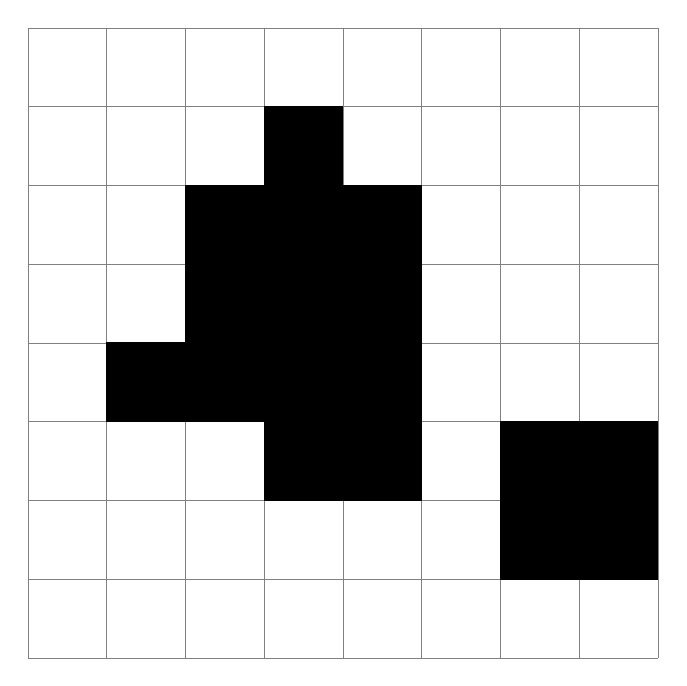
\begin{tikzpicture}
		\draw[help lines, step=1] (-4, -4) grid (4, 4);
		\foreach \x in {(-3, -1), (-2, -1), (-2, 0), (-2, 1), (-1, -2), (-1, -1), (-1, 0), (-1, 1), (-1, 2), (0, -2), (0, -1), (0, 0), (0, 1), (2, -3), (2, -2), (3, -3), (3, -2)}
			\filldraw[black] \x rectangle + (1, 1);
	\end{tikzpicture}
	\caption{Binary image, where the pixels with value one are black.}
	\label{exampleopeningbefore}
\end{figure}

Now, we apply morphological dilation to the eroded image. The result can be seen in figure \ref{exampleopeningopening}. The $2 \times 2$ pixel square has been eliminated, since it is smaller than the structuring element, that was used. Also, the edges of the larger connected region have been smoothed.

This effect of morphological opening makes it a great tool for the smoothing of edges and outlier elimination.\\

% Draw opening example after binary erosion:
\begin{figure}[t!]
	\centering
	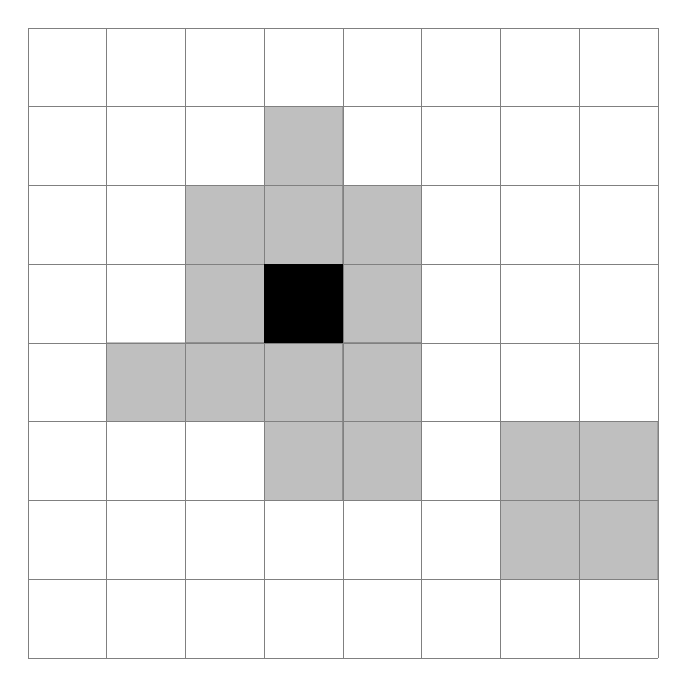
\begin{tikzpicture}
		\draw[help lines, step=1] (-4, -4) grid (4, 4);
		\foreach \x in {(-3, -1), (-2, -1), (-2, 0), (-2, 1), (-1, -2), (-1, -1), (-1, 0), (-1, 1), (-1, 2), (0, -2), (0, -1), (0, 0), (0, 1), (2, -3), (2, -2), (3, -3), (3, -2)}
			\filldraw[gray, opacity=0.5] \x rectangle + (1, 1);
		\foreach \x in {(-1, 0)}
			\filldraw[black] \x rectangle + (1, 1);
	\end{tikzpicture}
	\caption{Result of binary erosion of the image from figure \ref{exampleopeningbefore} with a $3 \times 3$ pixel structuring element. The transparent pixels are now set to zero.}
	\label{exampleopeningerosion}
\end{figure}

% Draw opening example after binary opening:
\begin{figure}[h!]
	\centering
	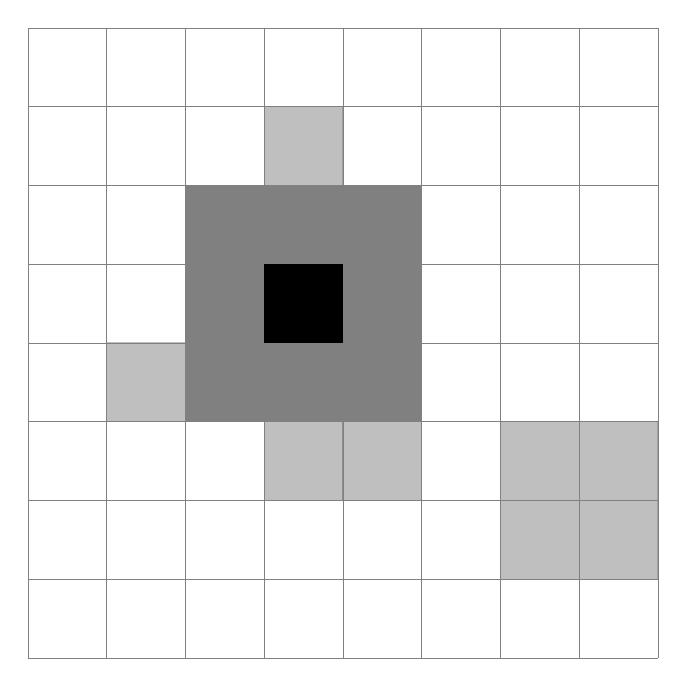
\begin{tikzpicture}
		\draw[help lines, step=1] (-4, -4) grid (4, 4);
		\foreach \x in {(-3, -1), (-1, -2), (-1, 2), (0, -2), (2, -3), (2, -2), (3, -3), (3, -2)}
			\filldraw[gray, opacity=0.5] \x rectangle + (1, 1);
		\foreach \x in {(-2, -1), (-2, 0), (-2, 1), (-1, -1), (-1, 0), (-1, 1), (0, -1), (0, 0), (0, 1)}
			\filldraw[gray] \x rectangle + (1, 1);
		\foreach \x in {(-1, 0)}
			\filldraw[black] \x rectangle + (1, 1);
	\end{tikzpicture}
	\caption{Binary image from figure \ref{exampleopeningbefore} after binary opening, i.e. erosion and dilation. The gray pixels were set to one again. Outliers have been eliminated and edges have been smoothed.}
	\label{exampleopeningopening}
\end{figure}

% ------------------------------------------------------------------------

Figure \ref{exampleclosingbefore} shows another example of a binary image. We want to perform morphological closing of this image. Again, we use a $3 \times 3$ pixel structuring element. First, morphological dilation is applied. The result of this can be seen in figure \ref{exampleclosingdilation}. The surrounding pixels of the four pixels, that had a value of one in the original image, have also been set to one by this morphological operation.

% Draw closing example before any morphological operations:
\begin{figure}[h]
	\centering
	
\begin{tikzpicture}
		\draw[help lines, step=1] (-4, -4) grid (4, 4);
		\foreach \x in {(-2, 0), (-2, 2), (1, 1), (1, -2)}
			\filldraw[black] \x rectangle + (1, 1);
	\end{tikzpicture}
	\caption{Binary image, where the pixels with value one are black.}
	\label{exampleclosingbefore}
\end{figure}

In a second step, morphological erosion is applied to the dilated image. The result can be seen in figure \ref{exampleclosingclosing}. The outer pixels are set to zero again, while the gaps between the four pixels, that had a value of one in the original image, have been filled.

For this reason, morphological closing is frequently used as a tool to fill gaps in binary images.

% Draw closing example after binary dilation:
\begin{figure}[t!]
	\centering
	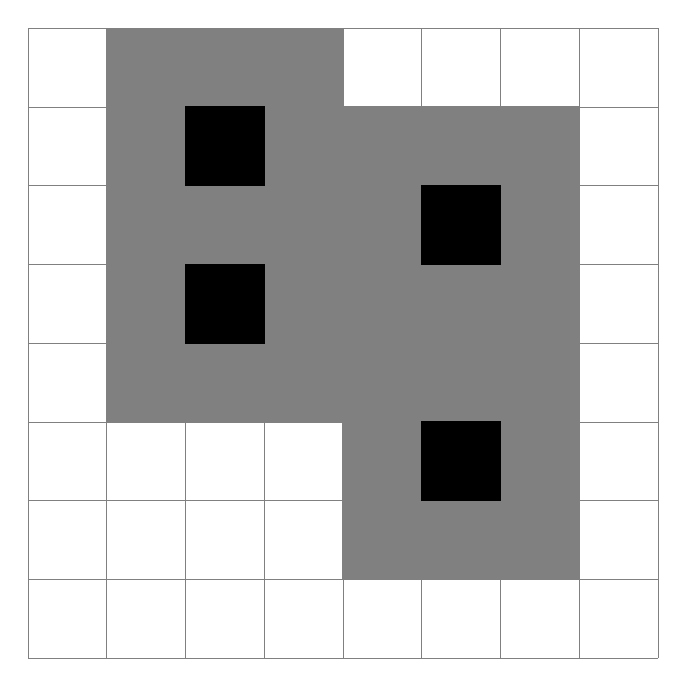
\begin{tikzpicture}
		\draw[help lines, step=1] (-4, -4) grid (4, 4);
		\foreach \x in {(-3, -1), (-3, 0), (-3, 1), (-3, 2), (-3, 3), (-2, -1), (-2, 0), (-2, 1), (-2, 2), (-2, 3), (-1, -1), (-1, 0), (-1, 1), (-1, 2), (-1, 3), (0, -3), (0, -2), (0, -1), (0, 0), (0, 1), (0, 2), (1, -3), (1, -2), (1, -1), (1, 0), (1, 1), (1, 2), (2, -3), (2, -2), (2, -1), (2, 0), (2, 1), (2, 2)}
			\filldraw[gray] \x rectangle + (1, 1);
		\foreach \x in {(-2, 0), (-2, 2), (1, 1), (1, -2)}
			\filldraw[black] \x rectangle + (1, 1);
	\end{tikzpicture}
	\caption{The image from figure \ref{exampleclosingbefore} after binary dilation with a $3 \times 3$ pixel structuring element. The gray pixels are now set to one.}
	\label{exampleclosingdilation}
\end{figure}

% Draw closing example after binary closing:
\begin{figure}[h!]
	\centering
	
\begin{tikzpicture}
		\draw[help lines, step=1] (-4, -4) grid (4, 4);
		\foreach \x in {(-3, -1), (-3, 0), (-3, 1), (-3, 2), (-3, 3), (-2, -1), (-2, 3), (-1, -1), (-1, 2), (-1, 3), (0, -3), (0, -2), (0, -1), (0, 2), (1, -3), (1, 2), (2, -3), (2, -2), (2, -1), (2, 0), (2, 1), (2, 2)}
			\filldraw[gray, opacity=0.5] \x rectangle + (1, 1);
		\foreach \x in {(-2, 0), (-2, 1), (-2, 2), (-1, 0), (-1, 1), (0, 0), (0, 1), (1, -2), (1, -1), (1, 0), (1, 1)}
			\filldraw[gray] \x rectangle + (1, 1);
		\foreach \x in {(-2, 0), (-2, 2), (1, 1), (1, -2)}
			\filldraw[black] \x rectangle + (1, 1);
	\end{tikzpicture}
	\caption{The result of binary closing of the image in figure \ref{exampleclosingbefore}, i.e. dilation and erosion. The transparent pixels are set to zero again. The gaps between pixels have been filled.}
	\label{exampleclosingclosing}
\end{figure}

% ------------------------------------------------------------------------

Altogether, both morphological opening and closing are effective tools to smooth edges. Morphological opening achieves this by eliminating outliers, while morphological closing fills gaps.

\newpage

\section{Main results}\label{sectionmainresults}

In sections \ref{sectionstatisticalsignificance} and \ref{sectionpower} we examined the probabilities of type I and II errors in the statistical test developed in section \ref{sectionstatisticalmodel}. We are interested in the change of these probabilities when morphological opening and closing are applied to the binarized image obtained as the outcome of the statistical test. One property of morphological opening and closing is $\Theta \circ \Psi \subseteq \Theta \subseteq \Theta \bullet \Psi$ for any structuring element $\Psi$. From this fact, we can deduce, that morphological opening will lower the probabiliy of a type I error, but increase the probability of a type II error. Morphological closing, on the other hand, will have the opposite effect. While this serves as a qualitative argument for the employment of these operators, we aim at quantifying this change of the probabilities. For this, we use a square structuring element, since we have the prior information, that the region of interest in the image is rectangular.
The next theorem states the change of the probability of a type I error after opening and after opening and closing with a square structuring element.

\begin{theorem}
	Let $m, n \in \mathbb{N}$, $c \in \mathbb{R} \setminus \{ 0 \}$ and $\Omega = \left\{ 1, \dots, m \right\} \times \left\{ 1, \dots, n \right\}$.
	
	Assume that $F$ follows the statistical model given in \eqref{image} and let $T(i, j)$ be the test statistic as defined in \eqref{teststatistic} and $H_0(i, j)$ be the null hypothesis as defined in \eqref{nullhypothesis}. Let $\alpha \in (0, 1)$ and $t_\alpha$ a threshold, such that
	\begin{equation*}
		\max \left\{ \mathbb{P}_V\left( \norm{\Delta^+ F(i, j)} \geq t_\alpha \right), \mathbb{P}_V\left( \norm{\Delta^- F(i, j)} \geq t_\alpha \right) \right\} \leq \alpha
	\end{equation*}
	for all $V \in \mathcal{H}_0(i, j)$. Let $\mathfrak{I}_\alpha$ be the binary image defined by
	\begin{equation}
		\mathfrak{I}_\alpha(i, j) = \mathds{1}_{ \{ T(i, j) \geq t_\alpha \} }
	\end{equation}
	for all $(i, j) \in \Omega$.
	
	Let $\varphi \in \mathbb{N}$ be odd. Let $\Phi_\varphi = \{ -\frac{\varphi - 1}{2}, -\frac{\varphi - 3}{2}, \dots, \frac{\varphi - 3}{2}, \frac{\varphi - 1}{2} \}$ and $\Psi_\varphi = \Phi_\varphi \times \Phi_\varphi$ be a structuring element. Let $(i, j) \in \Omega$ and $V \in \mathcal{H}_0(i, j)$.
	Then the following inequalities hold:
	\begin{align}
		\mathbb{P}_V( (\mathfrak{I}_\alpha \circ \Psi_\varphi)(i, j) = 1 ) &\leq \varphi \alpha^{\frac{\varphi + 1}{2}} \label{ineqtypeIopening} \\
		\mathbb{P}_V( ((\mathfrak{I}_\alpha \circ \Psi_\varphi) \bullet \Psi_\varphi)(i, j) = 1 ) &\leq \varphi^3 \alpha^{\frac{\varphi + 1}{2}} \label{ineqtypeIclosing}
	\end{align}
\end{theorem}
\begin{proof}
	We start with the proof of inequality \eqref{ineqtypeIopening}. We aim to find an upper bound for the probability
	\begin{equation*}
		\mathbb{P}_V( (\mathfrak{I}_\alpha \circ \Psi_\varphi)(i, j) = 1 )
	\end{equation*}
	for $V \in \mathcal{H}_0(i, j)$.
	
	We will perform some preparatory work first. As discussed in section \ref{sectiondefinitions}, any matrix $V \in \mathcal{V}_c^{m, n}$ is uniquely defined by the top left corner $(\kappa_1, \lambda_1)$ and bottom right corner $(\kappa_2, \lambda_2)$ of the rROI $\varLambda = \{ \kappa_1, \dots, \kappa_2 \} \times \{ \lambda_1, \dots, \lambda_2 \}$ contained in $V$.
	
	We have assumed, that $V \in \mathcal{H}_0(i, j)$. As we have seen in section \ref{sectionstatisticalmodel} the null hypothesis is equivalent to $(i, j) \notin \varLambda$. If $(i, j) \notin \varLambda$, this implies, that $i < \kappa_1$ or $j < \lambda_1$ or $i > \kappa_2$ or $j > \lambda_2$. These four cases are not mutually exclusive. We have also seen before, that the first two cases imply $\norm{\Delta^- V(i, j)} = 0$ and the latter two imply $\norm{\Delta^+ V(i, j)} = 0$.
	
	Based on this knowledge, we can split up the sets $\mathcal{H}_0^+(i, j)$ and $\mathcal{H}_0^-(i, j)$ as defined in \eqref{setH0+} and \eqref{setH0-}. We define the sets
	\begin{align*}
		\mathcal{H}_0^{(1)}(i, j) &\coloneqq \left\{ V \in \mathcal{V}_c^{m, n} \mid V(\tilde{i}, \tilde{j}) = 0 \textrm{ for all } (\tilde{i}, \tilde{j}) \in \{ 1, \dots, i \} \times \{ 1, \dots, n \} \right\} \\
		\mathcal{H}_0^{(2)}(i, j) &\coloneqq \left\{ V \in \mathcal{V}_c^{m, n} \mid V(\tilde{i}, \tilde{j}) = 0 \textrm{ for all } (\tilde{i}, \tilde{j}) \in \{ 1, \dots, m \} \times \{ 1, \dots, j \} \right\} \\
		\mathcal{H}_0^{(3)}(i, j) &\coloneqq \left\{ V \in \mathcal{V}_c^{m, n} \mid V(\tilde{i}, \tilde{j}) = 0 \textrm{ for all } (\tilde{i}, \tilde{j}) \in \{ i, \dots, m \} \times \{ 1, \dots, n \} \right\} \\
		\mathcal{H}_0^{(4)}(i, j) &\coloneqq \left\{ V \in \mathcal{V}_c^{m, n} \mid V(\tilde{i}, \tilde{j}) = 0 \textrm{ for all } (\tilde{i}, \tilde{j}) \in \{ 1, \dots, m \} \times \{ j, \dots, n \} \right\}
	\end{align*}
	and get $\mathcal{H}_0^-(i, j) = \mathcal{H}_0^{(1)}(i, j) \cup \mathcal{H}_0^{(2)}(i, j)$ and $\mathcal{H}_0^+(i, j) = \mathcal{H}_0^{(3)}(i, j) \cup \mathcal{H}_0^{(4)}(i, j)$. Furthermore, this implies $\mathcal{H}_0(i, j) = \bigcup_{u = 1}^4 \mathcal{H}_0^{(u)}(i, j)$.
	
	Depending on which of these sets $V$ belongs to, the rROI is located below/right of/above/left relative to the pixel $(i, j)$. This means, that all of the pixels above/left of/below/right of the index $(i, j)$ are not part of the rROI.
	
	Assume the first case, i.e. $V \in \mathcal{H}_0^{(1)}(i, j)$. This implies that
	\begin{equation*}
		\norm{\Delta^- V(i, 1)} = \ldots = \norm{\Delta^- V(i, n)} = 0
	\end{equation*}
	
	In a first step, we use equation \eqref{eqeventopening} and the fact, that $\Psi_\varphi = \Phi_\varphi \times \Phi_\varphi$ to write the left hand side of inequality \eqref{ineqtypeIopening} as
	\begin{align*}
		\mathbb{P}_V&( (\mathfrak{I}_\alpha \circ \Psi_\varphi)(i, j) = 1 ) \\
		&= \mathbb{P}_V\left( \bigcup_{(k, l) \in \Psi_\varphi} \bigcap_{(\tilde{k}, \tilde{l}) \in \Psi_\varphi} \{ \mathfrak{I}_\alpha(i - k + \tilde{k}, j - l + \tilde{l}) = 1 \} \right) \\
		&= \mathbb{P}_V\left( \bigcup_{k, l \in \Phi_\varphi} \bigcap_{\tilde{k}, \tilde{l} \in \Phi_\varphi} \{ \mathfrak{I}_\alpha(i - k + \tilde{k}, j - l + \tilde{l}) = 1 \} \right)
	\end{align*}
	
	Using sub-additivity we can bound this further from above by writing it as a sum over $l \in \Phi_\varphi$ and get
	\begin{align*}
		\mathbb{P}_V&( (\mathfrak{I}_\alpha \circ \Psi_\varphi)(i, j) = 1 ) \\
		&\leq \sum_{l \in \Phi_\varphi} \mathbb{P}_V\left( \bigcup_{k \in \Phi_\varphi} \bigcap_{\tilde{k}, \tilde{l} \in \Phi_\varphi} \{ \mathfrak{I}_\alpha(i - k + \tilde{k}, j - l + \tilde{l}) = 1 \} \right)
	\end{align*}
	
	By dropping every term except for $\tilde{k} = k$ in the intersection inside, we obtain
	\begin{align*}
		\mathbb{P}_V&( (\mathfrak{I}_\alpha \circ \Psi_\varphi)(i, j) = 1 ) \\
		&\leq \sum_{l \in \Phi_\varphi} \mathbb{P}_V\left( \bigcup_{k \in \Phi_\varphi} \bigcap_{\tilde{k} = k, \tilde{l} \in \Phi_\varphi} \{ \mathfrak{I}_\alpha(i - k + \tilde{k}, j - l + \tilde{l}) = 1 \} \right) \\
		&= \sum_{l \in \Phi_\varphi} \mathbb{P}_V\left( \bigcup_{k \in \Phi_\varphi} \bigcap_{\tilde{l} \in \Phi_\varphi} \{ \mathfrak{I}_\alpha(i, j - l + \tilde{l}) = 1 \} \right)
	\end{align*}
	
	The events inside the probability do not depend on $k \in \Phi_\varphi$ anymore, which yields
	\begin{equation*}
		\bigcup_{k \in \Phi_\varphi} \bigcap_{\tilde{l} \in \Phi_\varphi} \{ \mathfrak{I}_\alpha(i, j - l + \tilde{l}) = 1 \} = \bigcap_{\tilde{l} \in \Phi_\varphi} \{ \mathfrak{I}_\alpha(i, j - l + \tilde{l}) = 1 \}
	\end{equation*}
	
	By plugging this in, we obtain
	\begin{equation*}
		\mathbb{P}_V( (\mathfrak{I}_\alpha \circ \Psi_\varphi)(i, j) = 1 ) \leq \sum_{l \in \Phi_\varphi} \mathbb{P}_V\left( \bigcap_{\tilde{l} \in \Phi_\varphi} \{ \mathfrak{I}_\alpha(i, j - l + \tilde{l}) = 1 \} \right)
	\end{equation*}
	
	We have defined the binary $\mathfrak{I}_\alpha$ by setting $\mathfrak{I}_\alpha(i, j) = \mathds{1}_{ \{ T(i, j) \geq t_\alpha \} }$. Using this definition and the definition of $T(i, j)$ we can rewrite the upper bound as
	\begin{align*}
		&\sum_{l \in \Phi_\varphi} \mathbb{P}_V\left( \bigcap_{\tilde{l} \in \Phi_\varphi} \{ \mathfrak{I}_\alpha(i, j - l + \tilde{l}) = 1 \} \right) \\
		&= \sum_{l \in \Phi_\varphi} \mathbb{P}_V\left( \bigcap_{\tilde{l} \in \Phi_\varphi} \{ T(i, j - l + \tilde{l}) \geq t_\alpha \} \right) \\
		&= \sum_{l \in \Phi_\varphi} \mathbb{P}_V\left( \bigcap_{\tilde{l} \in \Phi_\varphi} \left( \{ \norm{\Delta^+ F(i, j - l + \tilde{l})} \geq t_\alpha \} \cap \{ \norm{\Delta^- F(i, j - l + \tilde{l})} \geq t_\alpha \} \right) \right)
	\end{align*}
	
	By dropping the events $\{ \norm{\Delta^+ F(i, j - l + \tilde{l})} \geq t_\alpha \}$, we get
	\begin{align*}
		\mathbb{P}_V&( (\mathfrak{I}_\alpha \circ \Psi_\varphi)(i, j) = 1 ) \\
		&\leq \sum_{l \in \Phi_\varphi} \mathbb{P}_V\left( \bigcap_{\tilde{l} \in \Phi_\varphi} \left( \{ \norm{\Delta^+ F(i, j - l + \tilde{l})} \geq t_\alpha \} \cap \{ \norm{\Delta^- F(i, j - l + \tilde{l})} \geq t_\alpha \} \right) \right) \\
		&\leq \sum_{l \in \Phi_\varphi} \mathbb{P}_V\left( \bigcap_{\tilde{l} \in \Phi_\varphi} \{ \norm{\Delta^- F(i, j - l + \tilde{l})} \geq t_\alpha \} \right)
	\end{align*}
	
	We now define a second set $\tilde{\Phi}_\varphi = \{ -\frac{\varphi - 1}{2}, -\frac{\varphi - 5}{2}, \dots, \frac{\varphi - 5}{2}, \frac{\varphi - 1}{2} \}$. We have $\tilde{\Phi}_\varphi \subseteq \Phi_\varphi$. Since $\Delta^- F(i, j)$ only depends on the pixels $(i, j), (i - 1, j), (i, j - 1)$, the set $\{ \norm{\Delta^- F(i, j - l + \tilde{l})} \mid \tilde{l} \in \tilde{\Phi}_\varphi \}$ is a set of independent random variables for fixed $l \in \Phi_\varphi$, see figure \ref{independentpoints}.
	
	% Draw picture of independent pixels:
	\begin{figure}[h]
		\centering
		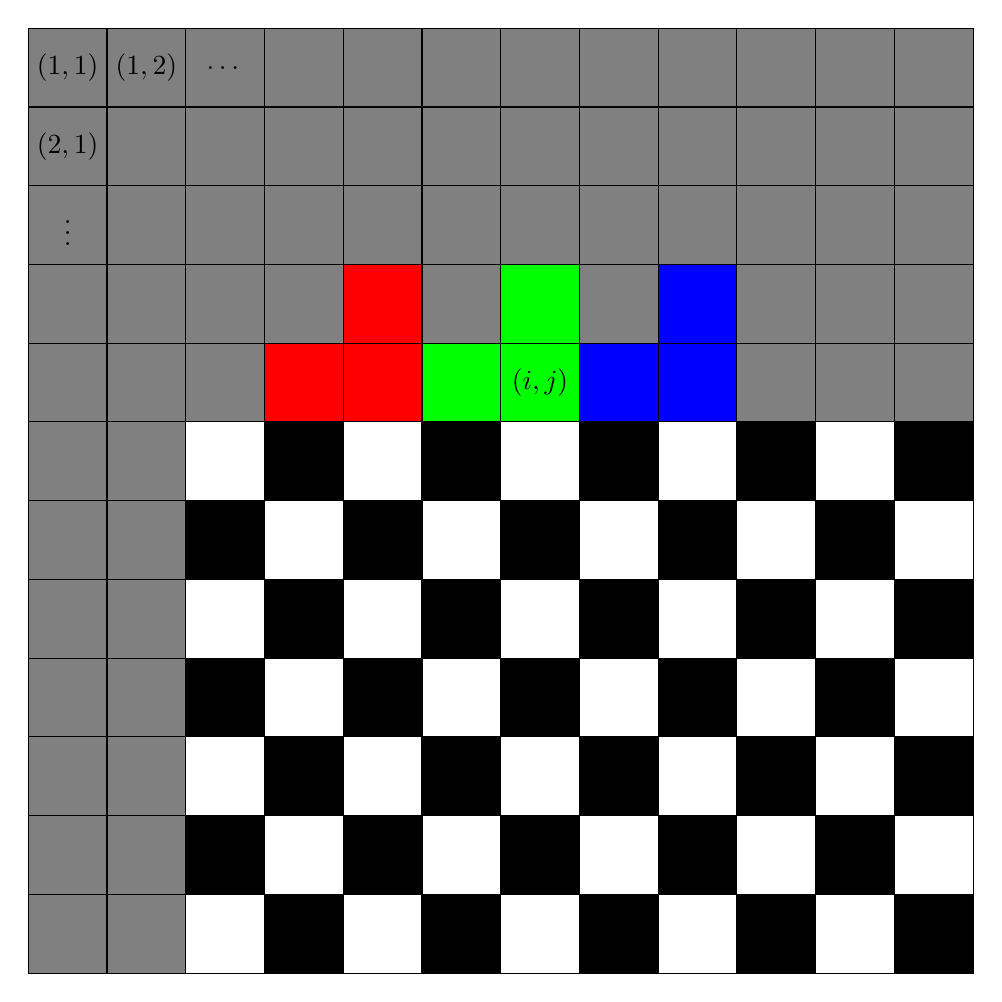
\begin{tikzpicture}
			\foreach \i in {-6, ..., 5}
				\foreach \j in {-6, ..., 5}
					\filldraw[gray] (\i, \j) rectangle + (1, 1);
			\foreach \i in {-4, ..., 5}
				\foreach \j in {-6, ..., 0}
					{
						\pgfmathparse{mod(\i+\j, 2) ? "black" : "white"}
						\edef\colour{\pgfmathresult}
						\filldraw[fill=\colour] (\i, \j) rectangle + (1, 1);
					}
			\foreach \x in {(-2, 1), (-3, 1), (-2, 2)}
				\filldraw[red] \x rectangle + (1, 1);
			\foreach \x in {(0, 1), (-1, 1), (0, 2)}
				\filldraw[green] \x rectangle + (1, 1);
			\foreach \x in {(2, 1), (1, 1), (2, 2)}
				\filldraw[blue] \x rectangle + (1, 1);
			\draw[step=1] (-6, -6) grid (6, 6);
			\node at (0.5, 1.5) {$(i, j)$};
			\node at (-5.5, 5.5) {$(1, 1)$};
			\node at (-4.5, 5.5) {$(1, 2)$};
			\node at (-3.5, 5.5) {$\dots$};
			\node at (-5.5, 4.5) {$(2, 1)$};
			\node at (-5.5, 3.5) {$\vdots$};
		\end{tikzpicture}
		\caption{The random variable $\norm{\Delta^- F(i, j)}$ only depends on the green pixels, $\norm{\Delta^- F(i, j - 2)}$ depends on the red pixels and $\norm{\Delta^- F(i, j + 2)}$ on the blue pixels. Since these are all distinct from another, the random variables are independent.}
		\label{independentpoints}
	\end{figure}
	
	We drop the terms in $\Phi_\varphi \setminus \tilde{\Phi}_\varphi$ and use the independence to obtain
	\begin{align*}
		\mathbb{P}_V( (\mathfrak{I}_\alpha \circ \Psi_\varphi)(i, j) = 1 ) &\leq \sum_{l \in \Phi_\varphi} \mathbb{P}_V\left( \bigcap_{\tilde{l} \in \Phi_\varphi} \{ \norm{\Delta^- F(i, j - l + \tilde{l})} \geq t_\alpha \} \right) \\
		&\leq \sum_{l \in \Phi_\varphi} \mathbb{P}_V\left( \bigcap_{\tilde{l} \in \tilde{\Phi}_\varphi} \{ \norm{\Delta^- F(i, j - l + \tilde{l})} \geq t_\alpha \} \right) \\
		&= \sum_{l \in \Phi_\varphi} \prod_{\tilde{l} \in \tilde{\Phi}_\varphi} \mathbb{P}_V\left( \norm{\Delta^- F(i, j - l + \tilde{l})} \geq t_\alpha \right)
	\end{align*}
	
	At the start of this proof, we have decomposed the set $\mathcal{H}_0(i, j)$ into four subsets. This was done by exploiting the prior knowledge, that $V$ contains a rectangular region of interest. We assumed the case $V \in \mathcal{H}_0^{(1)}(i, j)$, which means
	\begin{equation*}
		\norm{\Delta^- V(i, 1)} = \ldots = \norm{\Delta^- V(i, n)} = 0
	\end{equation*}
	
	This implies, that for fixed $l \in \Phi_\varphi$ the null hypotheses $H_0(i, j - l + \tilde{l})$ are true for all $\tilde{l} \in \tilde{\Phi}_\varphi$ and hence $V \in \bigcap_{\tilde{l} \in \tilde{\Phi}_\varphi} \mathcal{H}_0(i, j - l + \tilde{l})$. Furthermore, we have assumed, that the threshold $t_\alpha$ was chosen, such that for $V \in \mathcal{H}_0(i, j)$ we have $\mathbb{P}_V\left( \norm{\Delta^- F(i, j)} \geq t_\alpha \right) \leq \alpha$. Such a threshold can be obtained by using Lemma \ref{lemtypeIbound} and Theorem \ref{thmeqcdf}. This knowledge yields the upper bound
	\begin{align*}
		\mathbb{P}_V( (\mathfrak{I}_\alpha \circ \Psi_\varphi)(i, j) = 1 ) &\leq \sum_{l \in \Phi_\varphi} \prod_{\tilde{l} \in \tilde{\Phi}_\varphi} \mathbb{P}_V\left( \norm{\Delta^- F(i, j - l + \tilde{l})} \geq t_\alpha \right) \\
		&\leq \sum_{l \in \Phi_\varphi} \prod_{\tilde{l} \in \tilde{\Phi}_\varphi} \alpha \\
		&= \abs{\Phi_\varphi} \alpha^{\abs{\tilde{\Phi}_\varphi}} \\
		&= \varphi \alpha^{\frac{\varphi + 1}{2}}
	\end{align*}
	
	This proves the first inequality for the first case. The other three cases can be proven analogously by swapping the roles of $k$ or $\tilde{k}$ with $l$ or $\tilde{l}$, respectively and/or by replacing $\Delta^-$ by $\Delta^+$. This finishes the proof of the first inequality.\\
	
	
	For the proof of the second inequality, we want to exploit our prior knowledge on $V$ again. As already stated in the proof of the first inequality, we see, that $H_0(i, j)$ is equivalent to $(i, j) \notin \varLambda$, which is equivalent to at least one of the cases $V \in \mathcal{H}_0^{(u)}(i, j)$ for $u \in \{ 1, 2, 3, 4 \}$.
	
	Again we assume the first case, i.e. $V \in \mathcal{H}_0^{(1)}(i, j)$. This implies, that the null hypotheses $H_0(\tilde{i}, 1), \ldots, H_0(\tilde{i}, n)$ are true for all $\tilde{i} \in \{ 1, \dots, i \}$. It also implies
	\begin{equation*}
		\norm{\Delta^- V(\tilde{i}, 1)} = \ldots = \norm{\Delta^- V(\tilde{i}, n)} = 0
	\end{equation*}
	for all $\tilde{i} \in \{ 1, \dots, i \}$.
	
	Set $k_0 = -\frac{\varphi - 1}{2}$ and $l_0 = 0$. Then $(k_0, l_0) \in \Psi_\varphi$ and we get that the null hypotheses $H_0(i + k_0 - \tilde{k}, j + l_0 - \tilde{l})$ are true for all $\tilde{k}, \tilde{l} \in \Phi_\varphi$. Hence, we have $V \in \bigcap_{\tilde{k}, \tilde{l} \in \Phi_\varphi} \mathcal{H}_0(i + k_0 - \tilde{k}, j - \tilde{l})$ as well as $\norm{\Delta^- V(i + k_0 - \tilde{k}, j + l_0 - \tilde{l})} = 0$ for all $\tilde{k}, \tilde{l} \in \Phi_\varphi$.
	
	Define $\mathfrak{K}_\alpha = \mathfrak{I}_\alpha \circ \Psi_\varphi$. We use equation \eqref{eqeventclosing} and $\Psi_\varphi = \Phi_\varphi \times \Phi_\varphi$ to write the left hand side of inequality \eqref{ineqtypeIclosing} as
	\begin{align*}
		\mathbb{P}_V&( (\mathfrak{K}_\alpha \bullet \Psi_\varphi)(i, j) = 1 ) \\
		&= \mathbb{P}_V\left( \bigcap_{(k, l) \in \Psi_\varphi} \bigcup_{(\tilde{k}, \tilde{l}) \in \Psi_\varphi} \{ \mathfrak{K}_\alpha(i + k - \tilde{k}, j + l - \tilde{l}) = 1 \} \right) \\
		&= \mathbb{P}_V\left( \bigcap_{k, l \in \Phi_\varphi} \bigcup_{\tilde{k}, \tilde{l} \in \Phi_\varphi} \{ \mathfrak{K}_\alpha(i + k - \tilde{k}, j + l - \tilde{l}) = 1 \} \right)
	\end{align*}
	
	By dropping every term in the intersection except for $k = k_0$ and $l = l_0$ we can bound this from above by
	\begin{align*}
		\mathbb{P}_V( (\mathfrak{K}_\alpha \bullet \Psi_\varphi)(i, j) = 1 ) &= \mathbb{P}_V\left( \bigcap_{k, l \in \Phi_\varphi} \bigcup_{\tilde{k}, \tilde{l} \in \Phi_\varphi} \{ \mathfrak{K}_\alpha(i + k - \tilde{k}, j + l - \tilde{l}) = 1 \} \right) \\
		&\leq \mathbb{P}_V\left( \bigcup_{\tilde{k}, \tilde{l} \in \Phi_\varphi} \{ \mathfrak{K}_\alpha(i + k_0 - \tilde{k}, j + l_0 - \tilde{l}) = 1 \} \right) \\
		&= \mathbb{P}_V\left( \bigcup_{\tilde{k}, \tilde{l} \in \Phi_\varphi} \{ \mathfrak{K}_\alpha(i + k_0 - \tilde{k}, j - \tilde{l}) = 1 \} \right)
	\end{align*}
	
	Using sub-additivity to write this as the sum over all $\tilde{k}, \tilde{l} \in \Phi_\varphi$ yields
	\begin{equation*}
		\mathbb{P}_V( (\mathfrak{K}_\alpha \bullet \Psi_\varphi)(i, j) = 1 ) \leq \sum_{\tilde{k}, \tilde{l} \in \Phi_\varphi} \mathbb{P}_V\left( \mathfrak{K}_\alpha(i + k_0 - \tilde{k}, j - \tilde{l}) = 1 \right)
	\end{equation*}
	
	Plugging in the definition of $\mathfrak{K}_\alpha$ we obtain
	\begin{equation*}
		\mathbb{P}_V( (\mathfrak{K}_\alpha \bullet \Psi_\varphi)(i, j) = 1 ) \leq \sum_{\tilde{k}, \tilde{l} \in \Phi_\varphi} \mathbb{P}_V\left( (\mathfrak{I}_\alpha \circ \Psi_\varphi)(i + k_0 - \tilde{k}, j - \tilde{l}) = 1 \right)
	\end{equation*}
	
	As we have seen, the null hypotheses $H_0(i + k_0 - \tilde{k}, j + l_0 - \tilde{l})$ are true for all $\tilde{k}, \tilde{l} \in \Phi_\varphi$, which implies $V \in \bigcap_{\tilde{k}, \tilde{l} \in \Phi_\varphi} \mathcal{H}_0(i + k_0 - \tilde{k}, j - \tilde{l})$.
	
	Thus, we can use inequality \eqref{ineqtypeIopening} to get the upper bound
	\begin{align*}
		\mathbb{P}_V( (\mathfrak{K}_\alpha \bullet \Psi_\varphi)(i, j) = 1 ) &\leq \sum_{\tilde{k}, \tilde{l} \in \Phi_\varphi} \mathbb{P}_V\left( (\mathfrak{I}_\alpha \circ \Psi_\varphi)(i + k_0 - \tilde{k}, j - \tilde{l}) = 1 \right) \\
		&\leq \sum_{\tilde{k}, \tilde{l} \in \Phi_\varphi} \varphi \alpha^{\frac{\varphi + 1}{2}} \\
		&= \varphi^3 \alpha^{\frac{\varphi + 1}{2}}
	\end{align*}
	
	This proves the inequality in the first case. The other cases are proven analogously by taking $k_0 = 0, l_0 = -\frac{\varphi - 1}{2}$ in the second case, $k_0 = \frac{\varphi - 1}{2}, l_0 = 0$ in the third case and $k_0 = 0, l_0 = \frac{\varphi - 1}{2}$ in the fourth case. In the second and fourth case, the roles of $\Delta^+$ and $\Delta^-$ are swapped. This finishes the proof of the second inequality and thus the proof of the theorem.
\end{proof}

\newpage

\begin{theorem}
	Let $m, n \in \mathbb{N}$, $c \in \mathbb{R} \setminus \{ 0 \}$ and $\Omega = \left\{ 1, \dots, m \right\} \times \left\{ 1, \dots, n \right\}$.
	
	Assume that $F$ follows the statistical model given in \eqref{image} and let $T(i, j)$ be the test statistic as defined in \eqref{teststatistic} and $H_1(i, j)$ be the alternative hypothesis as defined in \eqref{alternativehypothesis}. Let $t$ be a threshold, such that
	\begin{equation*}
		\mathbb{P}_V\left( T(i, j) \leq t \right) \leq \beta
	\end{equation*}
	for all $V \in \mathcal{H}_1(i, j)$. Let $\mathfrak{I}$ be the binary image defined by
	\begin{equation}
		\mathfrak{I}(i, j) = \mathds{1}_{ \{ T(i, j) \geq t \} }
	\end{equation}
	for all $(i, j) \in \Omega$.
	
	Let $\varphi \in \mathbb{N}$ be odd. Let $\Phi_\varphi = \{ -\frac{\varphi - 1}{2}, -\frac{\varphi - 3}{2}, \dots, \frac{\varphi - 3}{2}, \frac{\varphi - 1}{2} \}$ and $\Psi_\varphi = \Phi_\varphi \times \Phi_\varphi$ be a structuring element. Let $(i, j) \in \Omega$ and $V \in \mathcal{H}_1(i, j)$.
	
	Denote by $\varLambda = \{ \kappa_1, \dots, \kappa_2 \} \times \{ \lambda_1, \dots, \lambda_2 \}$ the rROI contained in $V$. Let $\min \{ \kappa_2 - \kappa_1 + 1, \lambda_2 - \lambda_1 + 1 \} \geq \varphi$.
	Then the following inequalities hold:
	\begin{align}
		\mathbb{P}_V( (\mathfrak{I} \circ \Psi_\varphi)(i, j) = 0 ) &\leq \varphi^2 \beta \label{ineqtypeIIopening} \\
		\mathbb{P}_V( ((\mathfrak{I} \circ \Psi_\varphi) \bullet \Psi_\varphi)(i, j) = 0 ) &\leq \varphi^2 \beta \label{ineqtypeIIclosing}
	\end{align}
\end{theorem}
\begin{proof}
	We start by proving inequality \eqref{ineqtypeIIopening}. We use a similar approach as in the proof of inequality \eqref{ineqtypeIclosing} by finding indices $(k_0, l_0) \in \Psi_\varphi$, such that the alternative hypotheses $H_1(i - k_0 + \tilde{k}, j - l_0 + \tilde{l})$ are true for all $\tilde{k}, \tilde{l} \in \Phi_\varphi$. Define
	\begin{align*}
		k_0 &= \min \left\{ i - \kappa_1 - \frac{\varphi - 1}{2}, 0 \right\} - \min \left\{ \kappa_2 - i - \frac{\varphi - 1}{2}, 0 \right\} \\
		l_0 &= \min \left\{ j - \lambda_1 - \frac{\varphi - 1}{2}, 0 \right\} - \min \left\{ \lambda_2 - j - \frac{\varphi - 1}{2}, 0 \right\}
	\end{align*}
	
	First, we show, that $k_0$ can only take the values $i - \kappa_1 - \frac{\varphi - 1}{2}$, $- \kappa_2 + i + \frac{\varphi - 1}{2}$ or $0$. Then we distinguish the three possbile cases to show, that $\kappa_1 \leq i - k_0 + \tilde{k} \leq \kappa_2$ in every case. Similarly, we obtain $\lambda_1 \leq j - l_0 + \tilde{l} \leq \lambda_2$ and hence the alternative hypotheses $H_1(i - k_0 + \tilde{k}, j - l_0 + \tilde{l})$ are true for all $\tilde{k}, \tilde{l} \in \Phi_\varphi$.
	
	If $i - \kappa_1 - \frac{\varphi - 1}{2} \leq 0$, by using the assumption $\kappa_2 - \kappa_1 + 1 \geq \varphi$ we obtain
	\begin{align*}
		\kappa_2 - i - \frac{\varphi - 1}{2} &= \kappa_2 - i - \frac{\varphi - 1}{2} + \left( i - \kappa_1 - \frac{\varphi - 1}{2} \right) - \left( i - \kappa_1 - \frac{\varphi - 1}{2} \right) \\
		&= \kappa_2 - \kappa_1 + 1 - \varphi - i + \kappa_1 + \frac{\varphi - 1}{2} \\
		&\geq - i + \kappa_1 + \frac{\varphi - 1}{2} \\
		&\geq 0
	\end{align*}
	and thus $k_0 = i - \kappa_1 - \frac{\varphi - 1}{2}$. On the other hand, if $\kappa_2 - i - \frac{\varphi - 1}{2} \leq 0$, we obtain
	\begin{align*}
		i - \kappa_1 - \frac{\varphi - 1}{2} &= i - \kappa_1 - \frac{\varphi - 1}{2} + \left( \kappa_2 - i - \frac{\varphi - 1}{2} \right) - \left( \kappa_2 - i - \frac{\varphi - 1}{2} \right) \\
		&= \kappa_2 - \kappa_1 + 1 - \varphi - \kappa_2 + i + \frac{\varphi - 1}{2} \\
		&\geq - \kappa_2 + i + \frac{\varphi - 1}{2} \\
		&\geq 0
	\end{align*}
	and hence $k_0 = - \kappa_2 + i + \frac{\varphi - 1}{2}$, which shows, that $k_0$ can only take the values $i - \kappa_1 - \frac{\varphi - 1}{2}$, $- \kappa_2 + i + \frac{\varphi - 1}{2}$ or $0$.
	
	Assume $k_0 = 0$. This implies $i - \kappa_1 - \frac{\varphi - 1}{2} \geq 0$ as well as $\kappa_2 - i - \frac{\varphi - 1}{2} \geq 0$ and thus for $\tilde{k} \in \Phi_\varphi$ we get
	\begin{equation*}
		\kappa_1 \leq i - \frac{\varphi - 1}{2} \leq i + \tilde{k} = i - k_0 + \tilde{k} = i + \tilde{k} \leq i + \frac{\varphi - 1}{2} \leq \kappa_2
	\end{equation*}
	
	Now assume $k_0 = i - \kappa_1 - \frac{\varphi - 1}{2}$. Then $i - k_0 + \tilde{k} = \kappa_1 + \frac{\varphi - 1}{2} + \tilde{k}$. Using $\kappa_2 - \kappa_1 + 1 \geq \varphi$ yields for every $\tilde{k} \in \Phi_\varphi$
	\begin{align*}
		\kappa_1 &= \kappa_1 + \frac{\varphi - 1}{2} - \frac{\varphi - 1}{2} \\
		&\leq \kappa_1 + \frac{\varphi - 1}{2} + \tilde{k} \\
		&\leq \kappa_1 + \frac{\varphi - 1}{2} + \frac{\varphi - 1}{2} \\
		&= \kappa_1 + \varphi - 1 \\
		&\leq \kappa_2
	\end{align*}
	which proves the second case.
	
	Lastly, assume $k_0 = - \kappa_2 + i + \frac{\varphi - 1}{2}$. Then $i - k_0 + \tilde{k} = \kappa_2 - \frac{\varphi - 1}{2} + \tilde{k}$. Again, by $\kappa_2 - \kappa_1 + 1 \geq \varphi$ we obtain for every $\tilde{k} \in \Phi_\varphi$
	\begin{align*}
		\kappa_1 &\leq \kappa_2 - \varphi + 1 \\
		&= \kappa_2 - \frac{\varphi - 1}{2} - \frac{\varphi - 1}{2} \\
		&\leq \kappa_2 - \frac{\varphi - 1}{2} + \tilde{k} \\
		&\leq \kappa_2 - \frac{\varphi - 1}{2} + \frac{\varphi - 1}{2} \\
		&= \kappa_2
	\end{align*}
	
	Thus, the alternative hyptheses $H_1(i - k_0 + \tilde{k}, j - l_0 + \tilde{l})$ are true for all $\tilde{k}, \tilde{l} \in \Phi_\varphi$, which implies $V \in \bigcap_{\tilde{k}, \tilde{l} \in \Phi_\varphi} \mathcal{H}_1(i - k_0 + \tilde{k}, j - l_0 + \tilde{l})$.
	
	Using this, we can prove inequality \eqref{ineqtypeIIopening}. We start by using equation \eqref{eqeventopening} and $\Psi_\varphi = \Phi_\varphi \times \Phi_\varphi$ to write the left hand side of inequality \eqref{ineqtypeIIopening} as
	\begin{align*}
		\mathbb{P}_V( (\mathfrak{I} \circ \Psi_\varphi)(i, j) = 0 ) &= \mathbb{P}_V\left( \bigcap_{(k, l) \in \Psi_\varphi} \bigcup_{(\tilde{k}, \tilde{l}) \in \Psi_\varphi} \{ \mathfrak{I}(i - k + \tilde{k}, j - l + \tilde{l}) = 0 \} \right) \\
		&= \mathbb{P}_V\left( \bigcap_{k, l \in \Phi_\varphi} \bigcup_{\tilde{k}, \tilde{l} \in \Phi_\varphi} \{ \mathfrak{I}(i - k + \tilde{k}, j - l + \tilde{l}) = 0 \} \right)
	\end{align*}
	
	We drop every term in the intersection except $k = k_0, l = l_0$ to bound this further by
	\begin{align*}
		\mathbb{P}_V( (\mathfrak{I} \circ \Psi_\varphi)(i, j) = 0 ) &= \mathbb{P}_V\left( \bigcap_{k, l \in \Phi_\varphi} \bigcup_{\tilde{k}, \tilde{l} \in \Phi_\varphi} \{ \mathfrak{I}(i - k + \tilde{k}, j - l + \tilde{l}) = 0 \} \right) \\
		&\leq \mathbb{P}_V\left( \bigcup_{\tilde{k}, \tilde{l} \in \Phi_\varphi} \{ \mathfrak{I}(i - k_0 + \tilde{k}, j - l_0 + \tilde{l}) = 0 \} \right)
	\end{align*}
	
	We use sub-additivity to write this as the sum over all $\tilde{k}, \tilde{l} \in \Phi_\varphi$ and obtain
	\begin{equation*}
		\mathbb{P}_V( (\mathfrak{I} \circ \Psi_\varphi)(i, j) = 0 ) \leq \sum_{\tilde{k}, \tilde{l} \in \Phi_\varphi} \mathbb{P}_V\left( \mathfrak{I}(i - k_0 + \tilde{k}, j - l_0 + \tilde{l}) = 0 \right)
	\end{equation*}
	
	Using the fact, that $V \in \bigcap_{\tilde{k}, \tilde{l} \in \Phi_\varphi} \mathcal{H}_1(i - k_0 + \tilde{k}, j - l_0 + \tilde{l})$ as well as the definition of $\mathfrak{I}$ and the choice of the threshold $t$ we get the upper bound
	\begin{align*}
		\mathbb{P}_V( (\mathfrak{I} \circ \Psi_\varphi)(i, j) = 0 ) &\leq \sum_{\tilde{k}, \tilde{l} \in \Phi_\varphi} \mathbb{P}_V\left( \mathfrak{I}(i - k_0 + \tilde{k}, j - l_0 + \tilde{l}) = 0 \right) \\
		&= \sum_{\tilde{k}, \tilde{l} \in \Phi_\varphi} \mathbb{P}_V\left( T(i - k_0 + \tilde{k}, j - l_0 + \tilde{l}) \leq t \right) \\
		&\leq \sum_{\tilde{k}, \tilde{l} \in \Phi_\varphi} \beta \\
		&= \abs{\Phi_\varphi}^2 \beta \\
		&= \varphi^2 \beta
	\end{align*}
	
	This finishes the proof of the first inequality.\\
	
	
	To prove the second inequality, we define $\mathfrak{K} = \mathfrak{I} \circ \Psi_\varphi$. We aim to find an upper bound for the probability
	\begin{equation*}
		\mathbb{P}_V( (\mathfrak{K} \bullet \Psi_\varphi)(i, j) = 0 )
	\end{equation*}
	for $V \in \mathcal{H}_1(i, j)$. We use equation \eqref{eqeventclosing} and $\Psi_\varphi = \Phi_\varphi \times \Phi_\varphi$ and get
	\begin{align*}
		\mathbb{P}_V( (\mathfrak{K} \bullet \Psi_\varphi)(i, j) = 0 ) &= \mathbb{P}_V\left( \bigcup_{(k, l) \in \Psi_\varphi} \bigcap_{(\tilde{k}, \tilde{l}) \in \Psi_\varphi} \{ \mathfrak{K}(i + k - \tilde{k}, j + l - \tilde{l}) = 0 \} \right) \\
		&= \mathbb{P}_V\left( \bigcup_{k, l \in \Phi_\varphi} \bigcap_{\tilde{k}, \tilde{l} \in \Phi_\varphi} \{ \mathfrak{K}(i + k - \tilde{k}, j + l - \tilde{l}) = 0 \} \right)
	\end{align*}
	
	We drop every term in the intersection except for $\tilde{k} = k, \tilde{l} = l$. This increases the probability and we obtain
	\begin{align*}
		\mathbb{P}_V( (\mathfrak{K} \bullet \Psi_\varphi)(i, j) = 0 ) &= \mathbb{P}_V\left( \bigcup_{(k, l) \in \Psi_\varphi} \bigcap_{(\tilde{k}, \tilde{l}) \in \Psi_\varphi} \{ \mathfrak{K}(i + k - \tilde{k}, j + l - \tilde{l}) = 0 \} \right) \\
		&\leq \mathbb{P}_V\left( \bigcup_{k, l \in \Phi_\varphi} \bigcap_{\tilde{k} = k, \tilde{l} = l} \{ \mathfrak{K}(i + k - \tilde{k}, j + l - \tilde{l}) = 0 \} \right) \\
		&= \mathbb{P}_V\left( \bigcup_{k, l \in \Phi_\varphi} \{ \mathfrak{K}(i, j) = 0 \} \right) \\
		&= \mathbb{P}_V\left( \mathfrak{K}(i, j) = 0 \right)
	\end{align*}
	
	Plugging in the definition of $\mathfrak{K}$ this inequality becomes
	\begin{equation*}
		\mathbb{P}_V( (\mathfrak{K} \bullet \Psi_\varphi)(i, j) = 0 ) \leq \mathbb{P}_V( (\mathfrak{I} \circ \Psi_\varphi)(i, j) = 0 )
	\end{equation*}
	
	Since $V \in \mathcal{H}_1(i, j)$, we can apply inequality \eqref{ineqtypeIIopening} and obtain the upper bound
	\begin{align*}
		\mathbb{P}_V( (\mathfrak{K} \bullet \Psi_\varphi)(i, j) = 0 ) &\leq \mathbb{P}_V( (\mathfrak{I} \circ \Psi_\varphi)(i, j) = 0 ) \\
		&\leq \varphi^2 \beta
	\end{align*}
	
	This proves the second inequality and thus finishes the proof.
\end{proof}

\newpage

% Settings for Matlab code inclusion
\definecolor{mygreen}{rgb}{0,0.6,0}
\definecolor{mygray}{rgb}{0.5,0.5,0.5}
\definecolor{mymauve}{rgb}{0.58,0,0.82}
\lstset{ 
	backgroundcolor=\color{white},   % choose the background color; you must add \usepackage{color} or \usepackage{xcolor}; should come as last argument
	basicstyle=\footnotesize,        % the size of the fonts that are used for the code
	breakatwhitespace=false,         % sets if automatic breaks should only happen at whitespace
	breaklines=true,                 % sets automatic line breaking
	captionpos=b,                    % sets the caption-position to bottom
	commentstyle=\color{mygreen},    % comment style
	deletekeywords={...},            % if you want to delete keywords from the given language
	escapeinside={\%*}{*)},          % if you want to add LaTeX within your code
	extendedchars=true,              % lets you use non-ASCII characters; for 8-bits encodings only, does not work with UTF-8
	firstnumber=1,                	 % start line enumeration with line 1
	frame=single,	                 % adds a frame around the code
	keepspaces=true,                 % keeps spaces in text, useful for keeping indentation of code (possibly needs columns=flexible)
	keywordstyle=\color{blue},       % keyword style
	language=Matlab,                 % the language of the code
	morekeywords={*,...},            % if you want to add more keywords to the set
	numbers=left,                    % where to put the line-numbers; possible values are (none, left, right)
	numbersep=5pt,                   % how far the line-numbers are from the code
	numberstyle=\tiny\color{mygray}, % the style that is used for the line-numbers
	rulecolor=\color{black},         % if not set, the frame-color may be changed on line-breaks within not-black text (e.g. comments (green here))
	showspaces=false,                % show spaces everywhere adding particular underscores; it overrides 'showstringspaces'
	showstringspaces=false,          % underline spaces within strings only
	showtabs=false,                  % show tabs within strings adding particular underscores
	stepnumber=1,                    % the step between two line-numbers. If it's 1, each line will be numbered
	stringstyle=\color{mymauve},     % string literal style
	tabsize=2 	                     % sets default tabsize to 2 spaces
}

\begin{appendix}
	\section{Algorithms}
	
	\lstinputlisting[caption=\emph{MATLAB} implementation of a trial and error algorithm to find a threshold for the statistical test.]{ROI-Detection/ProbabilityDistribution/Threshold.m}
\end{appendix}


\newpage

% ------------------------------------------------------------------------



% ------------------------------------------------------------------------

\newpage

\addcontentsline{toc}{section}{References}
\bibliography{References}
\bibliographystyle{plain}


%\newpage
%
%\section*{Eidesstattliche Erklärung}
%\addcontentsline{toc}{section}{Eidesstattliche Erklärung}
%Ich erkläre, dass ich meine Master-Arbeit "`On the influence of morphological operators on testing for a region of interest"' selbstständig und ohne Benutzung anderer als der angegebenen Hilfsmittel angefertigt habe und dass ich alle Stellen, die ich wörtlich oder sinngemäß aus Veröffentlichungen entnommen habe, als solche kenntlich gemacht habe. Die Arbeit hat bisher in gleicher oder ähnlicher Form oder auszugsweise noch keiner Prüfungsbehörde vorgelegen.\\\\
%
%Ich versichere, dass die eingereichte schriftliche Fassung der auf dem beigefügten Medium gespeicherten Fassung entspricht.
%\\\\\\
%\noindent Göttingen, den \today
%\begin{flushright}
%	$\overline{~~~~~~~~~\mbox{(Dominik Blank)}~~~~~~~~~}$
%\end{flushright}













%\newpage
%
%\section{Multiple testing procedures}
%
%In a next step, we want to employ one of three multiple testing procedures. Consider the following setup:
%\begin{table}[h]
%	\tymax .3\textwidth
%	\begin{tabulary}{\textwidth}{|CCCC|}
%		\hline
%		& \textit{Declared non-significant} & \textit{Declared significant} & \textit{Total} \\
%		\hline
%		\textit{True null hypotheses} & $\mathbf{U}$ & $\mathbf{V}$ & $k_0$ \\
%		\textit{Non-true null hypotheses} & $\mathbf{T}$ & $\mathbf{S}$ & $m - k_0$ \\
%		& $m - \mathbf{R}$ & $\mathbf{R}$ & $m$ \\
%		\hline
%	\end{tabulary}
%\end{table}
%
%\begin{itemize}
%	\item $m$ is the total number hypotheses tested
%	\item $k_0$ is the number of true null hypotheses, an unknown parameter
%	\item $m - k_0$ is the number of true alternative hypotheses
%	\item $V$ is the number of false positives (Type I error) (also called "false discoveries")
%	\item $S$ is the number of true positives
%	\item $T$ is the number of false negatives (Type II error)
%	\item $U$ is the number of true negatives
%	\item $R = V + S$ is the number of rejected null hypotheses (also called "discoveries", either true or false)
%\end{itemize}
%In $m$ hypothesis tests of which $k_0$ are true null hypotheses, $\varLambda$ is an observable random variable, and $S$, $T$, $U$, and $V$ are unobservable random variables.
%
%We define another random variable $Q = \frac{V}{V + S}$, which is the proportion of the rejected null hypotheses which are erroneously rejected. We set $Q = 0$, if $V + S = 0$. Based on this, we define the false discovery rate to be
%\begin{equation}
%FDR = \mathbb{E}(Q) = \mathbb{E} \left( \frac{V}{V + S} \right)
%\end{equation}
%
%We also define the family-wise error rate to be
%\begin{equation}
%FWER = \mathbb{P}( V \geq 1 ) = 1 - \mathbb{P}( V = 0 )
%\end{equation}
%that is the probability of making one or more type I errors.
%
%Three of these multiple testing procedures are given in detail in the following. The first one controls the false discovery rate at level $\alpha$, i.e.
%\begin{equation}
%FDR = \mathbb{E}(Q) \leq \alpha
%\end{equation}
%
%The other two procedures control the family-wise error rate at level $\alpha$, i.e.
%\begin{equation}
%FWER = \mathbb{P}( V \geq 1 ) \leq \alpha
%\end{equation}
%
%First, we calculate for every pixel $(i, j) \in G$ the $p$-value
%\begin{equation}
%p(i, j) = \exp \left( - \frac{\tilde{d}(i, j)^2}{4 \sigma^2} \right) \geq \mathbb{P}(T \geq \tilde{d}(i, j) \mid H_0)
%\end{equation}
%
%\subsection{FDR Thresholding}
%\begin{enumerate}[(i)]
%	\item Sort $p$-values in ascending order: $p_{(1)} \leq p_{(2)} \leq \dots \leq p_{(M \cdot N)}$
%	\item Calculate the maximal index $k$, such that $p_{(k)} \leq \frac{k \cdot \alpha}{M \cdot N}$
%	\item Calculate the threshold $\lambda_{k} = 2 \sigma \sqrt{- \log(p_{(k)})}$
%	\item Reject all hypotheses $H_{(i)}$ with $p_{(i)} \leq p_{(k)}$, i.e. all hypotheses with $$\tilde{d}_{(i)} \geq \tilde{d}_{(k)} = \lambda_{k} = 2 \sigma \sqrt{- \log(p_{(k)})}$$
%\end{enumerate}
%
%\subsection{Bonferroni Thresholding}
%\begin{enumerate}[(i)]
%	\item Reject all hypotheses $H_{i}$ with $p_{i} \leq \frac{\alpha}{M \cdot N}$, i.e. all hypotheses with $$\tilde{d}_{i} \geq \lambda_k = 2 \sigma \sqrt{- \log \left( \frac{\alpha}{M \cdot N} \right)}$$
%\end{enumerate}
%
%\subsection{Hochberg Thresholding}
%\begin{enumerate}[(i)]
%	\item Sort $p$-values in ascending order: $p_{(1)} \leq p_{(2)} \leq \dots \leq p_{(M \cdot N)}$
%	\item Calculate the maximal index $k$, such that $p_{(k)} \leq \frac{\alpha}{M \cdot N - k + 1}$
%	\item Reject all hypotheses $H_{(i)}$ with $p_{(i)} \leq p_{(k)}$, i.e. all hypotheses with $$\tilde{d}_{(i)} \geq \tilde{d}_{(k)} = \lambda_{k} = 2 \sigma \sqrt{- \log(p_{(k)})}$$
%\end{enumerate}
%
%\begin{remark}
%	All these methods are defined for actual $p$-values, i.e.
%	\begin{equation*}
%	p(i, j) = \mathbb{P}(T \geq \tilde{d}(i, j) \mid H_0)
%	\end{equation*}
%	In contrast to that, we have taken upper bounds for the $p$-values. This is not an issue though, since by taking upper bounds we might decrease the number of hypotheses we reject. Thus it will not increase the error rate.
%\end{remark}
%
%\begin{remark}
%	The threshold has the following interpretation:
%	\begin{itemize}
%		\item If $\tilde{d}(i, j) \geq \lambda_{k}$, then $(i, j)$ is part of the ROI.
%		\item If $\tilde{d}(i, j) < \lambda_{k}$, then $(i, j)$ is NOT part of the ROI.
%	\end{itemize}
%\end{remark}
%
%\newpage
%
%\subsection{Example}
%\begin{figure}[h]
%	\includegraphics[width=\linewidth]{Thresholding_Comparison}
%	\caption[Comparison of different thresholding procedures]{The top left is the original image f of testDemo.mat, top right is the ROI with FDR thresholding, bottom left is the ROI with Bonferroni thresholding and bottom right is the ROI with Hochberg thresholding. (Standard deviation of the noise is $\sigma = 7$.)}
%	\label{fig:demo1comparison}
%\end{figure}

\end{document}
